\documentclass[pdflatex,sn-mathphys-num,iicol]{sn-jnl}
\usepackage{graphicx}
\usepackage{adjustbox}
\usepackage{booktabs}
\usepackage{array}
\usepackage{enumerate}
\usepackage{multirow}
\usepackage{xcolor}
\usepackage{microtype}
\usepackage{amsmath,amssymb}
\usepackage{amsthm}
\usepackage[section]{placeins}
\newtheorem{definition}{Definition}
\newtheorem{proposition}{Proposition}
\newtheorem{corollary}{Corollary}
\setcounter{topnumber}{5}
\setcounter{bottomnumber}{5}
\setcounter{totalnumber}{8}
\renewcommand{\topfraction}{0.90}
\renewcommand{\bottomfraction}{0.80}
\renewcommand{\textfraction}{0.07}
\renewcommand{\floatpagefraction}{0.75}
\raggedbottom
\providecommand{\jyear}[1]{}
\makeatletter
\@ifundefined{tableorg}{}{%
\let\table\tableorg
\let\endtable\endtableorg
\let\sidewaystable\sidewaystableorg
\let\endsidewaystable\endsidewaystableorg
}
\makeatother
\jyear{2026}

\title{Benchmark Collapse in Text CAPTCHAs: Generator Heterogeneity, Cross-Generator Transfer, and Reliability-Aware Synthetic Evaluation}

\author[1]{\fnm{Anonymous} \sur{Author}}

\affil[1]{\orgname{Institution withheld for peer review}, \orgaddress{\country{Anonymous}}}

\abstract{Text-based CAPTCHAs remain widely studied, but published results often depend as much on the benchmark generator as on the recognition model. We examine this problem under controlled synthetic conditions and make four contributions. First, we document a defect reported in the original CAPTCHA generation pipeline and replace that renderer with a controlled implementation. The original pre-repair image archive is unavailable, so we do not claim a reproducible quantitative re-run of that state; instead, we provide a reproducible audit of the corrected release and a separately labeled captcha-library proxy. Second, we construct CAPTCHA-X, a 160,000-image benchmark spanning four generators and four difficulty levels: \texttt{pil\_controlled}, \texttt{captcha\_image}, \texttt{opencv\_text}, and \texttt{wand\_text}. Third, under the fixed-slot protocol, classifiers show severe cross-generator instability: models exceeding 97\% and 99\% exact accuracy on matched \texttt{pil\_controlled} and \texttt{opencv\_text} medium sets fall below 6\% and 21\% on \texttt{captcha\_image} and \texttt{wand\_text}, showing that benchmark outcomes can be dominated by generator choice rather than model capability. Fourth, we report reliability diagnostics for exact accuracy, calibration error, out-of-distribution AUROC, abstention behavior, and a vulnerability score across all 4$\times$4 train/test transfers. Transfer is asymmetric and structured, no model generalizes meaningfully to \texttt{captcha\_image}, and calibration deteriorates sharply under transfer. The study is deliberately limited to synthetic images to isolate benchmark behavior under controlled conditions.}

\keywords{CAPTCHA; benchmark validity; generator diversity; cross-generator transfer; calibration; synthetic evaluation}


\begin{document}

\maketitle


% =============================================================
\section{Introduction}
% =============================================================

The core of the security claim for a text-based CAPTCHA is a claim about
measurements: namely, that it is harder for machines to transcribe than for
humans, making it an effective distinction between the two groups. But any such
claim will only be as credible as the benchmark against which the claim
is measured. Benchmarking in the area of CAPTCHA design does not usually
get the attention it deserves. Generator settings are presumed to match
their claimed difficulty level. Benchmarks are viewed as interchangeable.
Solve rates are compared across different studies that use different
generators, distortion methods, and vocabularies. This has created a
literature where results cannot be meaningfully compared, reproduced, or
interpreted.

The advances made by deep learning methods have drastically narrowed the performance gap between human and machine in solving text CAPTCHAs. Convolutional recurrent networks~\cite{shi2017crnn} and sequence models based on CTC decoding~\cite{graves2006ctc} achieve high accuracy on both synthetic and selected families of real-world CAPTCHAs, with GAN-boosted approaches demonstrating expanded attack effectiveness even under conditions of insufficiently labeled data~\cite{goodfellow2014generative,ye2018captcha,li2020endtoendcaptcha,aguilar2021captcha}. The trend of these results is well understood.

What remains uncertain, however, is how precise these claims actually are. Reported success rates are often not accompanied by explicit consideration of distribution shift, benchmark reliability, or the crucial difference between distribution-matched accuracy and true ability to break CAPTCHA. As a consequence, reproducibility, fair comparisons, and reasonable security estimations become impossible. At times, this is unintentional---benchmark design is rarely considered in discussions about CAPTCHA security. Overall, this approach leads to research results which cannot be independently validated.

In this regard, this paper aims to address the problem by starting at the beginning. The initial pipeline required validation of tensor handling, scheduler usage, and data labeling. During that process, contemporaneous diagnostics indicated that the renderer's advertised ``clean'' mode could contain nuisance marks. The pre-repair image archive is no longer available, so the present paper reports the corrected renderer and labels the available captcha-library row as a proxy rather than claiming a reproducible reconstruction.

\textbf{Contributions.} The contributions of this paper can be summarized as follows:

\begin{enumerate}
    \item \textbf{Generator Honesty Audit and Pixel-Level Verifier.}
    We document a defect reported in the original pipeline and replace that
    renderer with a controlled implementation. The original pre-repair image
    archive is unavailable, so we do not claim a reproducible quantitative
    re-run of that state. We instead provide a reproducible audit of the
    corrected release and a separately labeled captcha-library proxy, together
    with an explicit $(\varepsilon,\delta)$-honesty procedure.

    \item \textbf{CAPTCHA-X: A 160,000 Image Four-Generator Benchmark.}
    We develop and publish a synthetic benchmark of four rendering modes 
    (\texttt{pil\_controlled}, \texttt{captcha\_image},
    \texttt{opencv\_text}, \texttt{wand\_text}) $\times$ four levels of
    difficulty $\times$ 10,000 examples per condition with audited metadata.

\item \textbf{Four-by-Four Transfer Matrix on All Generators.}
    We train one fixed-slot model for each generator, run 64
    generator--difficulty evaluation conditions overall, and construct a
    $4 \times 4$ medium-difficulty transfer matrix from the resulting
    96,000 predictions. Generator transfer is asymmetric, structurally governed,
    and unpredictable based solely on accuracy against distributionally
    matched datasets.

    \item \textbf{Reliability Scorecard on Five Dimensions.}
    We introduce and empirically validate reliability diagnostics including
    exact accuracy, ECE, out-of-distribution AUROC, abstention utility, and
    a V-Score computed from exact accuracy, calibration, and entropy. Solve
    rate and calibration quality can be entirely unrelated, so accuracy alone
    is not a sufficient security metric.
\end{enumerate}

% =============================================================
\section{Related Work}
% =============================================================

\subsection{CAPTCHA Design and the Security Argument}

von Ahn et al.~\cite{vonahn2003captcha} formalized the CAPTCHA as a security primitive whose strength is derived from unresolved AI problems. The design logic was sound in 2003: if transcribing distorted text is hard for machines, it serves as a human-machine discriminant. As the survey by Guerar et al.~\cite{guerar2021captcha} documents across two decades of research, that logic has eroded progressively as each successive AI capability milestone has narrowed the gap.

Text CAPTCHAs responded with escalating distortion: rotation, shear, overlapping characters, clutter, occlusion, and background noise. The intent was to maintain human-machine asymmetry. But this strategy has two failure modes: it eventually harms human usability more than automated accuracy, and it assumes that distortion difficulty outpaces representation learning, which is increasingly questionable~\cite{guerar2021captcha,bursztein2014end}.

\subsection{Attack-Side Deep Learning}

The combination of convolutional visual encoding and CTC-based sequence decoding~\cite{lecun1998gradient,shi2017crnn,graves2006ctc,chen2017captcha} has proved highly effective for both scene text and distorted CAPTCHA strings. CRNN does not require explicit segmentation of characters, which is typically a huge challenge in attacks. Data augmentation through GANs as proposed~\cite{goodfellow2014generative,ye2018captcha} along with the use of an end-to-end attack pipeline as described~\cite{li2020endtoendcaptcha} has greatly expanded the attack vector and thus reduced the amount of data needed to create an effective attack model. Aguilar et al.~\cite{aguilar2021captcha} achieved very high accuracy for solving text-based CAPTCHAs using deep learning, particularly within a defense evaluation framework.

A common theme from the findings is that good generator assumptions are key factors behind the success: attacks that can generate enough samples from the target distribution or can use a synthetic generator similar to the production system can achieve much better results. Modern scene-text recognizers also make clear why an architecture check matters: ABINet~\cite{abinet2021}, VisionLAN~\cite{visionlan2021}, SVTR~\cite{svtr2022}, PARSeq~\cite{parseq2022}, and TrOCR~\cite{trocr2023} use language modeling, visual transformers, or variable-width sequence decoding rather than fixed slots. Our question is narrower than general domain generalization: WILDS~\cite{wilds2021} and DomainBed~\cite{domainbed2021} study distribution shifts across data sources, whereas CAPTCHA-X holds the label space and sampling protocol fixed and varies the renderer itself. The contribution is therefore an audit and transfer protocol for CAPTCHA benchmarks, not a claim that generator shift is a new form of distribution shift.

\subsection{Reliability in Neural Classifiers}

One common element absent in most works regarding attacks on CAPTCHAs is that of uncertainty analysis. Guo et al.~\cite{guo2017calibration} and Naeini et al.~\cite{naeini2015obtaining} have shown that current neural nets tend to overestimate their certainty, and that even simple post hoc calibration can significantly bring the two closer together. Hendrycks and Gimpel~\cite{hendrycks2017baseline}, Liang et al.~\cite{liang2018enhancing}, and Liu et al.~\cite{liu2020energy} set the foundation for out-of-distribution detection, which happens to be especially relevant to CAPTCHA evaluation, due to differing levels of distortion between contexts. Modern transformer architectures~\cite{vaswani2017attention,dosovitskiy2021vit} and advanced CNNs~\cite{liu2022convnext} provide improved foundation representations for reliability-oriented architectures.


\textbf{Positioning.} Table~\ref{tab:relatedwork} illustrates how this paper connects to several prior works. The key difference is not so much in architectural choices, but in the emphasis on benchmark honesty and reproducibility, as well as the focus on vulnerability assessment as opposed to solve rate.


\begin{table}[!htbp]
    \centering
    \caption{Positioning of this work relative to representative prior studies.}
    \label{tab:relatedwork}
    \resizebox{\columnwidth}{!}{%
    \begin{tabular}{p{1.8cm}p{2.7cm}p{3.3cm}}
        \toprule
        Work & Focus & Distinguishing feature \\
        \midrule
        von Ahn et al.~\cite{vonahn2003captcha} & Security primitive & Formal definition of CAPTCHA as an AI-hard security token \\
        Ye et al.~\cite{ye2018captcha} & Attack modeling &  Effective GAN-based solver, given favorable generator. \\
        Aguilar et al.~\cite{aguilar2021captcha} & Vulnerability assessment & Deep learning solver framed as a defensive analysis tool. \\
        This work & Reproducible benchmarking \& multi-generator transfer & Pipeline repair, generator honesty audit, cross-generator transfer evaluation, reliability components (ECE, OOD AUROC, abstention) validated experimentally. \\
        \bottomrule
    \end{tabular}
    }
\end{table}

% =============================================================
\section{Formal Definitions}
\label{sec:formal}
% =============================================================

We first present two formal definitions that support our empirical results.
Neither definition requires internal knowledge of the generator, and both can be tested empirically.

\begin{definition}[$(\varepsilon, \delta)$-Honest Generator]
Let $\mathcal{G}$ be a CAPTCHA generator and let $P$ be a difficulty
profile. Then $\mathcal{G}$ is called an $(\varepsilon, \delta)$-honest
generator with respect to $P$, where $\varepsilon > 0$ and $\delta \in [0, 1]$,
if
\begin{equation}
  \Pr_{x \sim \mathcal{G}(P)}\!\left[
    \bigl\|\phi(x) - \phi_P\bigr\|_2 > \varepsilon
  \right] < \delta,
\end{equation}
where $\phi(x)$ is a feature vector representing some form of distortion in
image $x$ (e.g., pixel variance, frequency energy, stroke discontinuities).
For a reproducible cross-family audit, $\phi_P$ is fixed before testing as the
coordinate-wise median of 1,000 images produced by the corrected PIL renderer
at profile $P$, using the same image size, alphabet, and seed. The prescribed
vector contains normalized background standard deviation, background
high-frequency FFT ratio, and foreground-pixel fraction; all components are
scaled to $[0,1]$. Thus $\varepsilon=0.01$ is a Euclidean distance on this
normalized vector, and $\delta$ is the observed flagged fraction. The
available legacy reports predate this reference-vector calculation and report
the raw-pixel/FFT flag separately in Table~\ref{tab:verifier}; they should not
be read as measurements of the new distance. The reference is never estimated
from the tested generator's own outputs.
\end{definition}

\noindent A generator is said to be dishonest if there is non-negligible probability
that the images generated by the benchmark do not conform to their
difficulty claim. Section~\ref{sec:honesty} reports the available provenance evidence and the
closest current clean captcha-library proxy. The original pre-repair images and
verifier log are not available, so this proxy does not reproduce the original
quantitative baseline.

\begin{definition}[Collapse of Benchmark]
A CAPTCHA benchmark $\mathcal{B}$ suffers from the problem of \emph{collapse}
under model $M$ trained on generator $\mathcal{G}$ if
\begin{equation}
  A_{\mathrm{exact}}(M,\, \mathcal{G}_{\mathrm{train}}=\mathcal{G},\,
  \mathcal{G}_{\mathrm{test}}=\mathcal{G}) > \tau_{\mathrm{human}},
\end{equation}
where $\tau_{\mathrm{human}}$ is human exact-match accuracy on $\mathcal{B}$,
and $M$ was trained on less than $n^*$ images and for less than $e^*$ epochs,
with the thresholds $n^*, e^*$ much smaller than those required by the
complexity of the task.
\end{definition}

\noindent The collapse phenomenon does \emph{not} correspond to model failure:
It can arise when structural regularities introduced by a generator match the fixed-slot preprocessing. The empirical high-accuracy result at $n^*=5{,}600$ and $e^*=3$ on \texttt{pil\_controlled} is presented in Section~\ref{sec:results}. The low scores on \texttt{captcha\_image} and \texttt{wand\_text} are interpreted as interactions between their rendering geometry and this recognizer, not as properties of the generators for arbitrary architectures.

\begin{proposition}[Operational indicators of fixed-slot collapse]
\label{thm:collapse}
For the fixed-slot model, we use the following three operational indicators when interpreting a collapse-like result. They are diagnostic conditions, not a sufficiency theorem:
\begin{enumerate}[(i)]
  \item \textbf{Positional regularity:} $\mathrm{Var}[\mathrm{xpos}_k(x)] <
        \sigma^2_{\mathrm{slot}}$ for all character positions $k$, where
        $\sigma^2_{\mathrm{slot}}$ is the slot half-width squared. This
        condition formalizes the fixed-width character assumption implicit
        in slot-based text recognizers~\cite{shi2017crnn}.
  \item \textbf{Character independence:} $I(c_k;\, c_j \mid x) \approx 0$
        for $k \neq j$. This is satisfied when characters are rendered
        independently without ligatures or overlapping strokes, as in most
        synthetic CAPTCHA generators~\cite{vonahn2003captcha,ye2018captcha}.
  \item \textbf{Low effective alphabet complexity:}
        $K\log |\mathcal{V}| / n_{\mathrm{train}}$ is small relative to the
        training protocol. We report this as a descriptive sample-complexity
        ratio; no universal generator-specific $\kappa$ is asserted.
\end{enumerate}
\end{proposition}
We evaluate these indicators empirically where the required measurements are available. We did not estimate $I(c_k;c_j\mid x)$, so condition (ii) is a rendering assumption rather than a measured information-theoretic quantity. We report the character-width coefficient of variation only for the captcha-image diagnostic (0.1228); comparable values for the other generators were not collected. Accordingly, these indicators support an architectural interpretation but do not establish generator-level sufficient conditions.
\noindent\textit{Remark.} We do not claim Proposition~\ref{thm:collapse} as a
proved theoretical result. It is an empirical diagnostic checklist for
separating positional mismatch from a failure to optimize the fixed-slot
solver, and it should be tested against additional architectures.

The indicators are consistent with the high fixed-slot accuracies on
\texttt{opencv\_text} and \texttt{pil\_controlled}; the available evidence does not show that they are sufficient, nor does it establish a generator-only effect.
For \texttt{captcha\_image}, proportional-width rendering increases character-width
variability and weakens positional regularity, as analyzed in
Section~\ref{sec:captcha_image_diagnosis}. For \texttt{wand\_text}, wave-like
distortion similarly disrupts the positional assumptions required by the
fixed-slot architecture.
% =============================================================
\section{Generator Honesty Audit and Pixel-Level Verification}
\label{sec:honesty_section}
% =============================================================

Before proceeding to describe the new benchmark's technical characteristics, it is important to describe the flaw in the original design which has made the benchmark interpretation impossible for the researchers building CAPTCHA evaluations based on an external renderer.

In the first dataset release, the rendering module consisted of the Python \texttt{captcha} library renderer~\cite{captcha_lib}. As mentioned earlier, the CAPTCHA library provided distortion parameters -- rotation, shear, line clutter and dot density -- which could be configured as zero, thereby allowing one to create a ``clean'' baseline. The underlying assumption, also present in the dataset metadata and release documentation, was that by setting the aforementioned parameters to zero, one could produce distortion-free images.

The assumption turned out to be false. The analysis of the images generated by the renderer with all distortion parameters set to zero showed that the nuisance marks were produced internally by the renderer and were not influenced by the specific parameters' settings. The metadata stated that there was zero clutter, but the pixel data indicated otherwise. This resulted in the fact that the ``clean'' split learned from images with different difficulty from the one described, affected the reproducibility of the accuracy metric according to the given configuration and made difficulty comparisons between the clean and noisy images impossible due to contamination of the baseline.

The corrective action was to replace the renderer with a PIL implementation that generates CAPTCHA images character-by-character, allowing explicit control of visual appearance. The resulting ``clean'' profile produces images which are truly clean -- fixed size, grayscale, no rotation, shear, clutter lines, dots, blur and noise. All of the distortion parameters used during rendering of every sample are tracked and reported in the metadata CSV file. Figure~\ref{fig:examples} presents samples from the new clean benchmark.

\begin{figure}[!htbp]
    \centering
    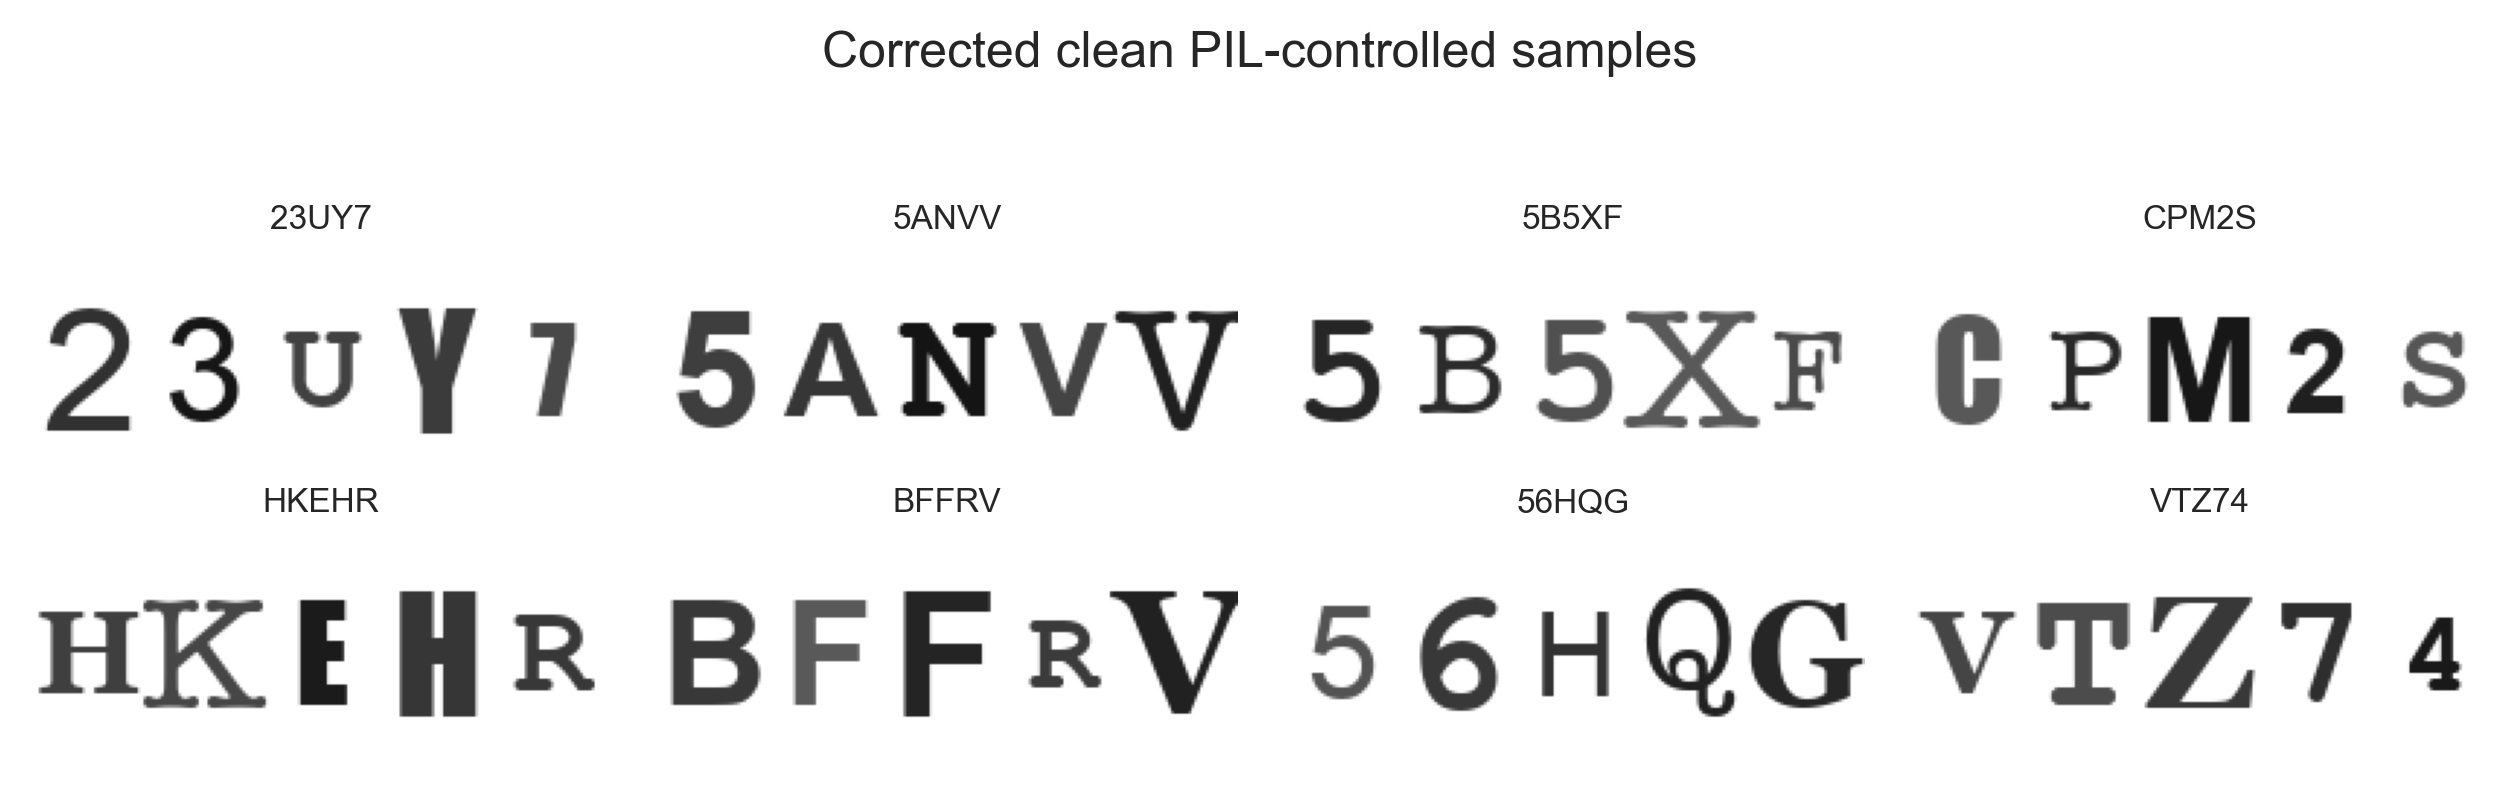
\includegraphics[width=\columnwidth]{figures/benchmark_examples.png}
    \caption{Representative samples of the corrected clean benchmark are shown below. These are images containing a five-character string chosen from the set of 32 characters and created without any geometric distortions, clutter, blurring, or additive noise. This can be discerned based on the data contained in the metadata CSV file. }
    \label{fig:examples}
\end{figure}

This solution has important methodological implications in that it necessitates the verification of benchmark cleanliness on a pixel-to-pixel basis as opposed to an estimate made by means of parameterization. When we consider CAPTCHA research, which tends to look at generators as black boxes based on parameterized hardness, such an issue can go unnoticed.

\subsection{Pixel-Level Verification Results}
\label{sec:honesty}

Table~\ref{tab:verifier} reports the available audit output. The original
pre-repair image archive and its verifier log were not preserved, so the
reported captcha-library row is a proxy and not a literal reconstruction of
the original baseline. We report mean pixel standard deviation only as a
luminance/stroke-coverage diagnostic, not as a distortion-energy estimate.
The ``flagged'' column is the legacy verifier's conservative raw-pixel/FFT flag (background standard deviation $>2.5$ on the
$0$--$255$ scale or background FFT ratio $>0.18$); it should not be read as
a direct measurement of the normalized $\varepsilon$ distance above.

\begin{table}[!htbp]
\centering
\caption{Pixel-level verification results for the corrected \texttt{pil\_controlled}
generator and the closest available captcha-library clean reference.
Mean pixel standard deviation $\bar{\sigma}_{\mathrm{px}}$ is reported as a
luminance/stroke-coverage diagnostic, together with the fraction of samples flagged as
clean-mismatch by the verifier. The current artifact set does not include a
separately archived pre-repair original-generator verification run, so
\texttt{captcha\_image}@clean is reported as the closest available clean
captcha-library measurement rather than as a literal pre-repair baseline.}
\label{tab:verifier}
\resizebox{\columnwidth}{!}{%
\begin{tabular}{llcc}
\toprule
Generator & Profile & $\bar{\sigma}_{\mathrm{px}}$ & Flagged (\%) \\
\midrule
\texttt{captcha\_image}  & clean  & 38.6260 & 65.4 \\
\texttt{pil\_controlled} & clean  & 71.1550 & 0.0 \\
\texttt{pil\_controlled} & easy   & 70.9123 & 0.0 \\
\texttt{pil\_controlled} & medium & 69.1136 & 0.0 \\
\texttt{pil\_controlled} & hard   & 66.4742 & 0.0 \\
\bottomrule
\end{tabular}
}
\end{table}
% =============================================================
\section{Proposed Methodology}
\label{sec:framework}
% =============================================================

\subsection{Overview}

CAPTCHA-X consists of the following pipeline stages: (1) Controlled generation with auditable difficulty metadata; (2) Preprocessing and normalization; (3) Training of models; (4) Evaluation through exact string and character comparison; and (5) Research on model robustness and reliability. The current implementation provides a CRNN baseline and a fixed-slot model. The present full-scale matrix uses the fixed-slot model; the reduced CRNN pilot reported in Section~\ref{sec:results} tests architecture sensitivity.

\begin{figure*}[!t]
    \centering
    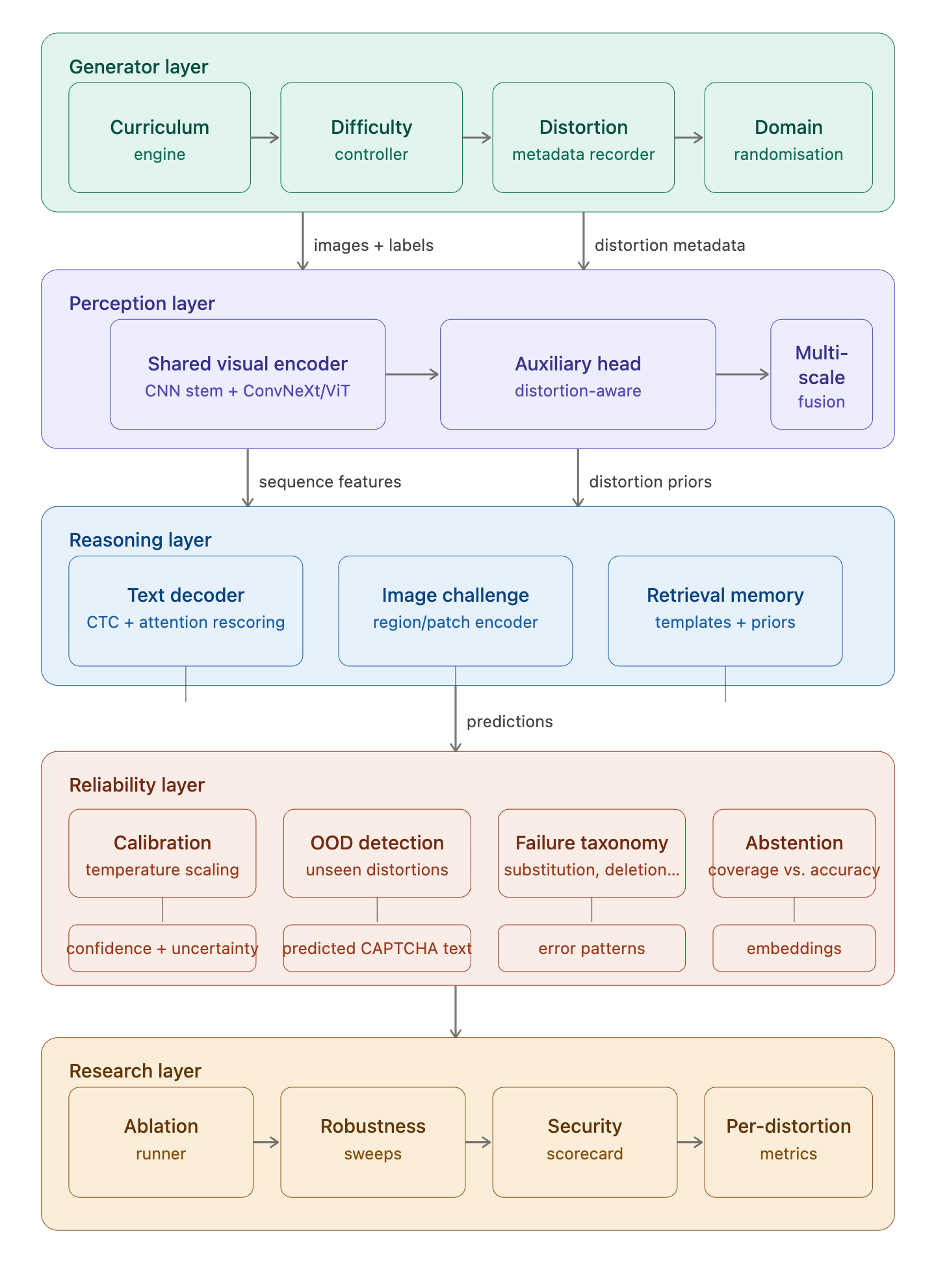
\includegraphics[width=\textwidth,height=0.42\textheight,keepaspectratio]{figures/captchaxarch.png}
    \caption{Layered architecture for CAPTCHA-X. The generator and text-recognition path are implemented and validated in the current paper. The reliability and research layers define the next stage: calibration, out-of-distribution detection, abstention policies, and per-distortion scorecards.}
    \label{fig:architecture}
\end{figure*}


\subsection{Controlled Synthetic Generator}

The repaired generator allows four difficulty profiles (named clean, easy, medium, hard), customizable character vocabulary, and logging of metadata per sample. The default character vocabulary consists of


\begin{equation}
\mathcal{V} = \{\texttt{2,3,4,5,6,7,8,9,A,\ldots,Z}\} \setminus \{\texttt{I,O,1,0}\},
\label{eq:vocab}
\end{equation}

resulting in $|\mathcal{V}| = 32$ symbols. The omission of visually ambiguous characters (O/0, I/1) is an industry best practice in CAPTCHA deployment and prevents the solvability of the test by humans from being compromised by visually indistinguishable characters.

The parameters of the difficulty profiles include maximum rotation (degrees), maximum shear, line-clutter count, dot count, Gaussian blur $\sigma$, and character spatial jitter. For the clean profile used in the core benchmark, these parameters are all set to zero, and the generated image is checked for any distortions.

\subsection{Preprocessing}

All input images are converted to grayscale, resized to the canonical size of $200\times80$, normalized to $[0,1]$ range, and polarity inverted such that foreground characters become dark strokes on a light background. This preprocessing step is applied uniformly across all difficulty profiles to decouple model architecture and distortion strength.

\subsection{CRNN Baseline}

CRNN baseline improvement~\cite{shi2017crnn} conforms to the classical structure of the convolutional encoder network~\cite{lecun1998gradient}, bidirectional RNN layers, and ultimately, the connectionist temporal classification decoder~\cite{graves2006ctc}. The geometry-related tensor problems with the original baseline code were resolved, the scheduler interface compatibility with the current PyTorch version was established, and an end-to-end pipeline of the full training cycle was successfully verified. This version of baseline code was created specifically for synthetic experimental testing purposes, including variation in string length and difficulty profile of generated samples.

\subsection{Fixed-Slot Benchmark Model}

The classifier we used as a clean benchmark for the controlled experiment consists of a fixed slot classifier based on the deterministic layout of fixed size CAPTCHAs. It partitions a normalized image into five overlapping horizontal crops, each corresponding to a certain letter position, and applies the same CNN classifier to each of them. The CNN crop classifier contains four convolutional layers from the classical CNN family~\cite{lecun1998gradient} followed by batch normalization, GELU activations, adaptive pooling, and two fully connected layers forming the head, consistent with modern deep vision practice~\cite{he2016deep}. Each crop overlaps the neighboring ones with a ratio of 0.25 of the nominal slot size to help with minor position jitter.

In doing so, we introduce a trade-off, where the resulting model is more specialized than the CRNN benchmark since it makes assumptions about the number of characters in the CAPTCHA and their position. However, such a model serves as a good upper bound on performance for the controlled experiment setting. It can also be interpreted as the security measure of an adversary knowing the size of the generated string and its vocabulary and cropping individual characters from it by position.

% =============================================================
\section{Experimental Design}
% =============================================================

\subsection{Problem Scope and Threat Model}

The experiments address offline vulnerability assessment: given the ability to sample from the target generator, how well can a matched model solve the task? We do not evaluate against live deployed services. The threat model is explicitly limited to:

\begin{itemize}
    \item a text CAPTCHA generator with known vocabulary, fixed string length, and controllable distortion;
    \item training on offline synthetic samples from the same distribution;
    \item evaluation on held-out samples from the identical benchmark configuration.
\end{itemize}

This is the appropriate threat model for measuring matched-distribution vulnerability. If a CAPTCHA is fragile under these conditions, that is a design-level finding regardless of whether deployment friction provides additional practical protection. On the other hand, if one gets such a result, there is no information on how it will behave when the data distribution changes.


\subsection{Benchmark Configuration}

The core benchmark contains 8{,}000 synthetic five-character CAPTCHAs created using the fixed renderer model. Its split is 5{,}600 training / 1{,}600 validation / 800 test. Table~\ref{tab:benchmark} documents both the core and full-scale configurations.

\begin{table}[!htbp]
\centering
\caption{Full-scale benchmark configuration across all four generator families.
All distortion parameters are verified at the pixel level via the honesty
verifier (Section~\ref{sec:honesty}). This constitutes the CAPTCHA-X benchmark.}
\label{tab:benchmark}
\resizebox{\columnwidth}{!}{%
\begin{tabular}{ll}
\toprule
Parameter & Value \\
\midrule
Image resolution & $200 \times 80$ \\
String length & 5 \\
Character vocabulary & 32 symbols ($\mathcal{V}$, Equation~\ref{eq:vocab}) \\
Generators & \texttt{pil\_controlled}, \texttt{captcha\_image},
             \texttt{opencv\_text}, \texttt{wand\_text} \\
Difficulty levels & Clean, Easy, Medium, Hard \\
Images per generator--difficulty & 10,000 \\
Total images & 160,000 \\
Full-scale train / val / test ratio & 70\% / 15\% / 15\% \\
Full-scale split (per condition) & 7,000 / 1,500 / 1,500 \\
Seed & 17 \\
Evaluation conditions & 64 ($4 \times 4 \times 4$) \\
Total predictions evaluated & 96,000 \\
Device & PyTorch 2.11.0, Apple MPS \\
\midrule
\multicolumn{2}{l}{\textit{Core benchmark (pil\_controlled, clean only)}} \\
\midrule
Total samples & 8,000 \\
Core split & 5,600 / 1,600 / 800 \\
\bottomrule
\end{tabular}
}
\end{table}

\subsection{Training Setup}

The fixed-slot classifier was trained with AdamW~\cite{loshchilov2019decoupled}, learning rate $10^{-3}$, batch size 256, hidden width 256, dropout rate 0.1, crop width 48, and overlap ratio 0.25. Training ran on Apple Metal Performance Shaders (MPS). The best checkpoint was saved by validation exact accuracy. The 10,000-image headline matrix uses seed 17. A separate reduced pilot (3,000 images per generator-condition; 1,000/200/200 train/validation/test) was run for seeds 17, 42, 99, 123, and 256 on the pil-controlled/opencv-text diagonal and associated transfer cells. We report its mean and standard deviation in the new architecture/seed-sensitivity paragraph; these estimates do not replace the full-scale seed-17 results.

\subsection{Evaluation Metrics}

Exact string accuracy is considered the main measure:
\begin{equation}
A_{\text{exact}} = \frac{1}{N}\sum_{i=1}^{N}\mathbb{1}[\hat{y}_i = y_i],
\end{equation}
where $\hat{y}_i$ is the predicted string and $y_i$ is the true answer. In the case of transcribing CAPTCHAs, exact string accuracy becomes the crucial measure: one misrecognition leads to a failure.

The secondary metric is character accuracy:
\begin{equation}
A_{\text{char}} = \frac{\sum_{i=1}^{N}\sum_{j=1}^{|y_i|}\mathbb{1}[\hat{y}_{i,j}=y_{i,j}]}{\sum_{i=1}^{N}|y_i|}.
\end{equation}

String accuracy complements character accuracy as the latter allows understanding the type of errors that have occurred. It provides information about whether the whole string was not recognized or whether there is one character mismatch.

For reliability metrics, confidence for a five-character prediction is the geometric mean of the five per-slot maximum softmax probabilities. Entropy is the mean of the five categorical entropies after temperature scaling, measured in nats and normalized by $\log |\mathcal{V}|$ to lie in $[0,1]$. ECE uses these sequence-level confidences and exact-string correctness with 15 equal-width bins. Temperature is a positive scalar applied by dividing logits; it is not an accuracy ratio.
% =============================================================
\section{Results}
\label{sec:results}
% =============================================================

\subsection{Training Dynamics}

Table~\ref{tab:history} summarizes the training behavior per epoch. The model reaches more than 95\% exact accuracy on validation in epoch 2 and reaches 0.9994 by epoch 3 in this recorded run. This rapid convergence is expected, considering that the task is not difficult for the same reason discussed earlier -- namely, identical distribution (fixed size, shape, no distortion, finite alphabet [32 characters]).

\begin{table}[!htbp]
    \centering
    \caption{Training history on the controlled clean benchmark. The model converges to near-perfect validation accuracy within three epochs.}
    \label{tab:history}
    \resizebox{\columnwidth}{!}{%
    \begin{tabular}{ccccc}
        \toprule
        Epoch & Train Loss & Train $A_{\text{char}}$ & Val $A_{\text{char}}$ & Val $A_{\text{exact}}$ \\
        \midrule
        1 & 1.0797 & 0.9006 & 0.8939 & 0.5663 \\
        2 & 0.0244 & 0.9906 & 0.9909 & 0.9563 \\
        3 & 0.0057 & 1.0000 & 0.9999 & 0.9994 \\
        \bottomrule
    \end{tabular}
    }
\end{table}
\subsection{Architecture-family and seed-sensitivity pilot}
We attempted an architecture-family check with the implemented CRNN on a reduced matched protocol (1,000/200/200 medium images per generator for train/validation/test, three epochs). The pilot did not reach non-zero exact accuracy before the planned stop, so we do not use it as evidence that the fixed-slot pattern survives a second architecture; the pilot summaries and logs are retained as a negative convergence result. Across the separate five-seed fixed-slot pilot for the two principal generators, matched-medium exact accuracy was $0.941\pm0.047$ for \texttt{opencv\_text} and $0.549\pm0.171$ for \texttt{pil\_controlled}; seed variation is therefore material and is now reported rather than hidden by Wilson intervals. A full-scale converged CRNN transfer matrix remains necessary future work.

\subsection{Diagnosis of Structural Resistance to Collapse: \texttt{captcha\_image}}
\label{sec:captcha_image_diagnosis}

The almost zero exact match accuracy on \texttt{captcha\_image} for the
fixed-slot model, independent of difficulty levels
(Table~\ref{tab:matched_gen_full}), needs explaining; this is not an indication
that \texttt{captcha\_image} is more difficult for human solvers, but that
\texttt{captcha\_image}'s font makes the positional regularities of the fixed-slot
model less true.

When analyzing the diagnostic report of the archived medium-difficulty
\texttt{captcha\_image}, one can conclude that \texttt{captcha\_image} relies
on a proportional font generator, where the character width is not uniform,
but depends on the glyph itself. The mean value of the character-width proxy
measured is 37.7496 pixels, while the standard deviation is 4.6346, the
variance proxy is 21.4797, and the coefficient of variation is 0.1228.
This variability can make fixed crops poorly centered for some glyphs. It is
evidence about the interaction between this renderer and this slot geometry;
we did not collect the corresponding width statistic for the other generators.

\textbf{Implication for Proposition~\ref{thm:collapse}:} the positional regularity requirement becomes weaker relative to the structurally regular generators that exhibit the phenomenon of collapse. This diagnostic supports a structural-mismatch interpretation, but it does not
prove that a general recognizer would fail. With 7,000 medium-difficulty
training examples, the fixed-slot model reaches 3.60\% on the corresponding
1,500-image test set. Across the six trained fixed-slot models evaluated on
\texttt{captcha\_image}@medium, 54 of 6,000 predictions are correct; among the
5,946 incorrect predictions, 5,891 are substitutions (99.08\%), 51 are
repeated-character errors (0.86\%), and 4 are transpositions (0.07\%). Confidence-based abstention cannot bail out a mismatched architecture. For \texttt{captcha\_image}@medium, the maximum selective accuracy at at
least 50\% coverage is 5.37\% at 60.87\% coverage (913 of 1,500 images), and with confidence threshold 0.99 no examples are left by the model at all. This is consistent with an interaction between proportional-width rendering and the fixed-slot preprocessing; it does not show that a general sequence recognizer would fail on this generator.
Namely, not only the overall complexity is too high,
but also the model crops do not correspond to the variable width generated by the generator.

\subsection{Held-Out Test Performance}

The held-out test set contains 800 samples; the top checkpoint obtains 99.875\% exact string accuracy and 99.975\% character accuracy. There are 4{,}000 total characters in the test set (5 per image $\times$ 800 images), meaning that 99.975\% character accuracy equates to one single character error. Table~\ref{tab:final} summarizes the final results.


\begin{table}[!htbp]
    \centering
    \caption{Final performance on the corrected clean benchmark (held-out test set). Metrics are sourced from the stored evaluation summary \texttt{slot\_classifier\_summary.json}.}
    \label{tab:final}
    \begin{tabular}{lc}
        \toprule
        Metric & Value \\
        \midrule
        Best validation $A_{\text{exact}}$ & 99.9375\% \\
        Test $A_{\text{exact}}$ & 99.8750\% \\
        Test $A_{\text{char}}$ & 99.9750\% \\
        Test samples & 800 \\
        Best epoch & 3 \\
        \bottomrule
    \end{tabular}
\end{table}

\subsection{Interpretation: What This Result Does and Does Not Show}

The 99.875\% figure is from the separate 8,000-image core benchmark (5,600/1,600/800 split), whereas the full-scale medium-trained \texttt{pil\_controlled}@clean result is 99.67\% on 1,500 test images. These are different protocols and should not be conflated. The 99.875\% figure is impressive, but its implications are limited. Specifically, it does not suggest that a deployed CAPTCHA system can be broken in this fraction of attempts. Nevertheless, it confirms three important aspects:

\begin{enumerate}
    \item For matching synthetic data, a straightforward architecture is enough to solve the problem almost perfectly. The hardness level has been reduced.
    \item Reduction occurred only in response to fixing the benchmark. In other words, a generator with misleading distortion metadata makes objective measurement of difficulty impossible.
    \item Only three epochs of training on a 5{,}600-sample core set were necessary to achieve these results. The low data and computational requirements point to another critical vulnerability: these results suggest that solving structurally uniform synthetic CAPTCHA families under matched conditions requires relatively modest computational resources.
\end{enumerate}

From the defender's perspective, the takeaway message is clear. Structural regularity is an insecure assumption even if there is no distortion. Introducing a minimal amount of distortion will increase the solve threshold, but the critical questions are by how much, under what conditions, and relative to what human baseline. The reliability-aware evaluation framework introduced in Section~\ref{sec:architecture} enables these questions to be studied more rigorously.
% =============================================================
\section{Cross-Generator Transfer Analysis and Reliability Evaluation}
\label{sec:local_extension}
% =============================================================

The formal collapse analysis from Section~\ref{sec:formal} presents an upper bound for
a single well-controlled generator in the setting of matched distribution.
The logical next step to take would be determining whether the observed
fragility and difficulty collapse phenomenon generalizes to other families
of renderers, or whether it is specific to one particular generator.
This section describes the second layer of experiments conducted using
entirely locally synthesized data; none of the live services, external
endpoints, or CAPTCHA providers were involved at any step.

\subsection{Experimental Setup}

Four local text-CAPTCHA generator backends are considered in the full-scale
extension: \texttt{pil\_controlled}, \texttt{captcha\_image} (Python
\texttt{captcha} library renderer~\cite{captcha_lib}),
\texttt{opencv\_text}, and \texttt{wand\_text}. For each generator, four
difficulty settings (clean, easy, medium, hard) are used with the same
32-symbol alphabet $\mathcal{V}$ defined in Section~\ref{sec:framework}.

For each generator--difficulty condition, 10,000 samples are generated with
seed 17 and split into 7,000 training, 1,500 validation, and 1,500 test
examples. One fixed-slot classifier is trained per generator on the
medium-difficulty split using the same architectural family as in the core
benchmark. Each trained model is then evaluated on all four difficulty levels
of all four generators, yielding a full $4 \times 4$ transfer matrix at
medium difficulty and 64 evaluation conditions overall. Thus ``matched
means matched generator, not matched difficulty: every row in the difficulty
sweep is evaluated by a model trained on that generator's medium split.
Figure~\ref{fig:gen_examples}
provides some examples for each generator backend.

\begin{figure}[!htbp]
    \centering
    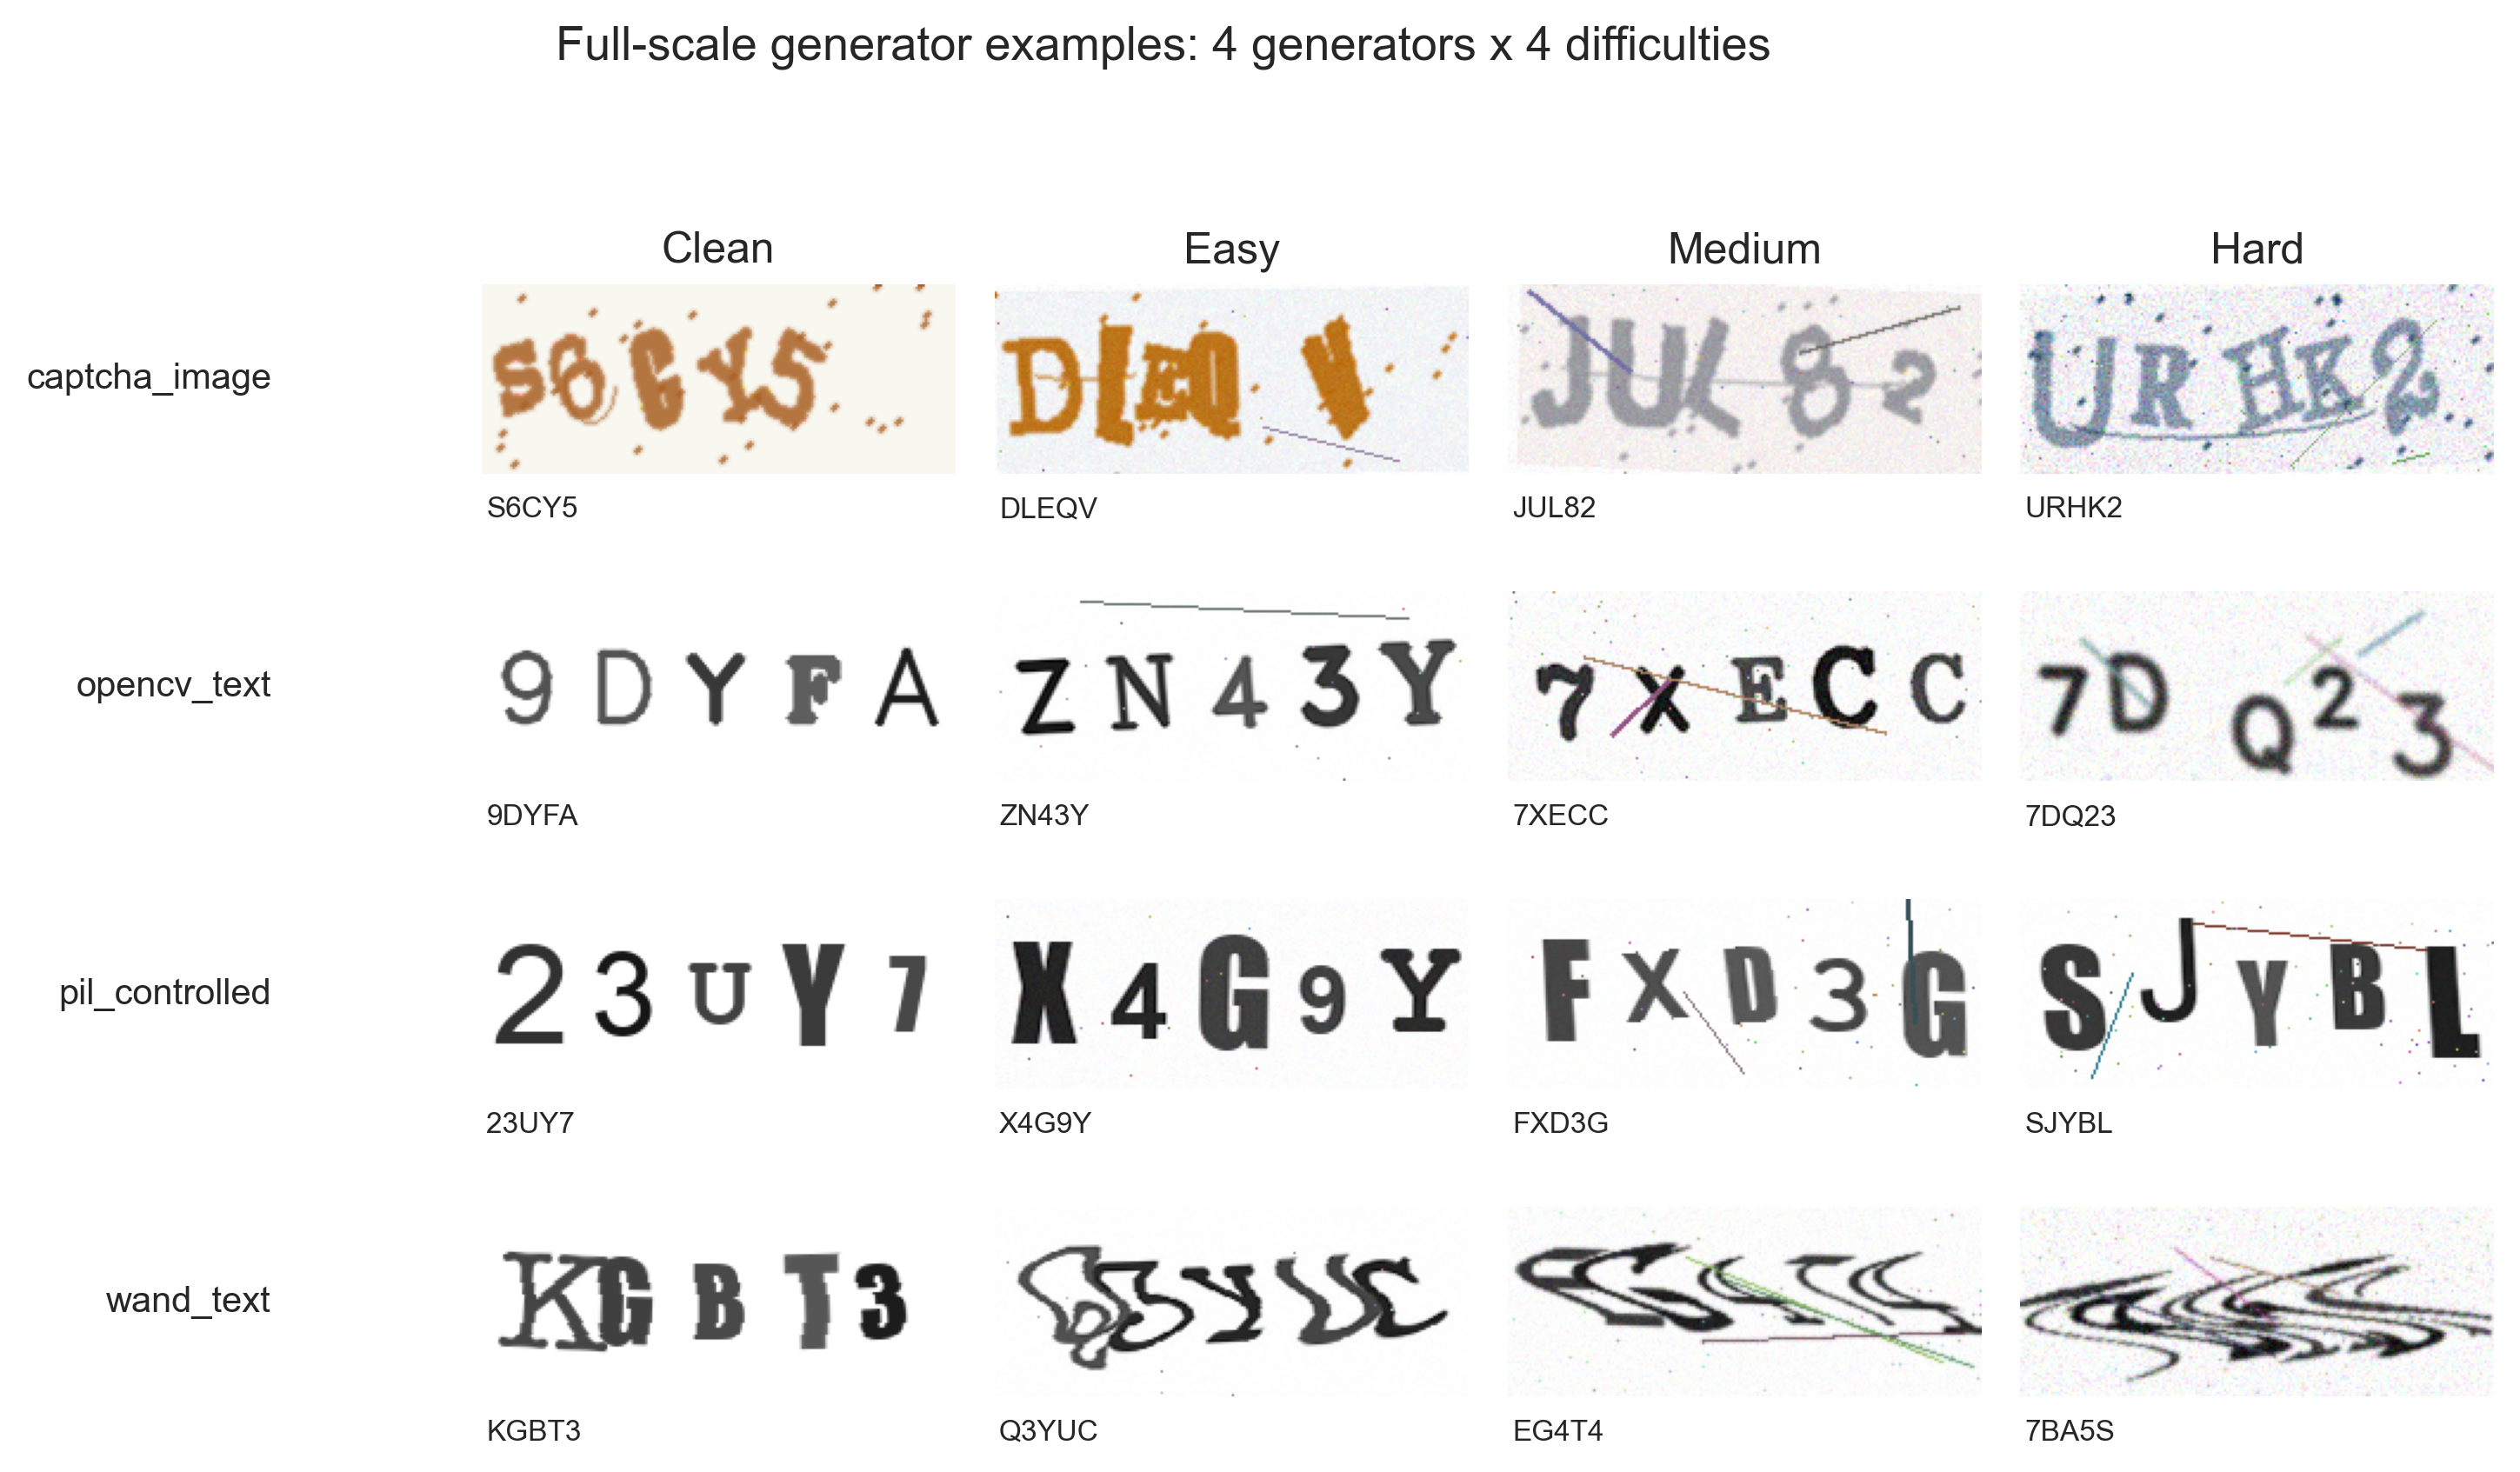
\includegraphics[width=\columnwidth]{figures/local_generator_examples.png}
    \caption{Representative samples from the four local generator backends
    (\texttt{pil\_controlled}, \texttt{captcha\_image}, \texttt{opencv\_text},
    and \texttt{wand\_text}) across benchmark difficulty levels. Despite identical vocabulary
    and string length, visual structure, stroke characteristics, and spatial
    layout differ substantially across families. All images are locally
    generated; no live service is involved.}
    \label{fig:gen_examples}
\end{figure}

\subsection{Matched-Generator Results}
\label{sec:matched}

Table~\ref{tab:matched_gen_full} shows the exact accuracy, character accuracy,
and ECE values obtained from the four matched-generator benchmark families for all levels
of difficulty. Figure~\ref{fig:exact_acc_diff} depicts these accuracy vs. difficulty trends.
\begin{table}[!htbp]
\centering
\caption{Evaluation with matched generators: full results from four renderer
families at four difficulty levels. $A_{\mathrm{exact}}$,
$A_{\mathrm{char}}$, and ECE scores are provided based on 1,500 test cases per
condition. Training data is derived from medium difficulty cases of the same
generator architecture.  Bold values indicate conditions where $A_{\mathrm{exact}} \geq 0.97$.}
\label{tab:matched_gen_full}
\resizebox{\columnwidth}{!}{%
\begin{tabular}{llccc}
\toprule
Generator & Difficulty & $A_{\mathrm{exact}}$ & $A_{\mathrm{char}}$ & ECE \\
\midrule
\multirow{4}{*}{\texttt{opencv\_text}}
    & Clean  & \textbf{1.0000} & \textbf{1.0000} & 0.0001 \\
    & Easy   & \textbf{0.9993} & \textbf{0.9999} & 0.0006 \\
    & Medium & \textbf{0.9980} & \textbf{0.9996} & 0.0015 \\
    & Hard   & 0.8987 & 0.9765 & 0.0851 \\
\midrule
\multirow{4}{*}{\texttt{pil\_controlled}}
    & Clean  & \textbf{0.9967} & \textbf{0.9993} & 0.0017 \\
    & Easy   & \textbf{0.9860} & \textbf{0.9972} & 0.0109 \\
    & Medium & \textbf{0.9727} & \textbf{0.9945} & 0.0197 \\
    & Hard   & 0.8480 & 0.9661 & 0.1224 \\
\midrule
\multirow{4}{*}{\texttt{wand\_text}}
    & Clean  & 0.4907 & 0.8663 & 0.2917 \\
    & Easy   & 0.4893 & 0.8653 & 0.2836 \\
    & Medium & 0.2080 & 0.6724 & 0.4301 \\
    & Hard   & 0.0693 & 0.3816 & 0.4116 \\
\midrule
\multirow{4}{*}{\texttt{captcha\_image}}
    & Clean  & 0.0553 & 0.5188 & 0.3382 \\
    & Easy   & 0.0540 & 0.5087 & 0.3383 \\
    & Medium & 0.0360 & 0.4737 & 0.3520 \\
    & Hard   & 0.0180 & 0.4171 & 0.3668 \\
\bottomrule
\end{tabular}
}
\end{table}

\begin{figure}[!htbp]
    \centering
    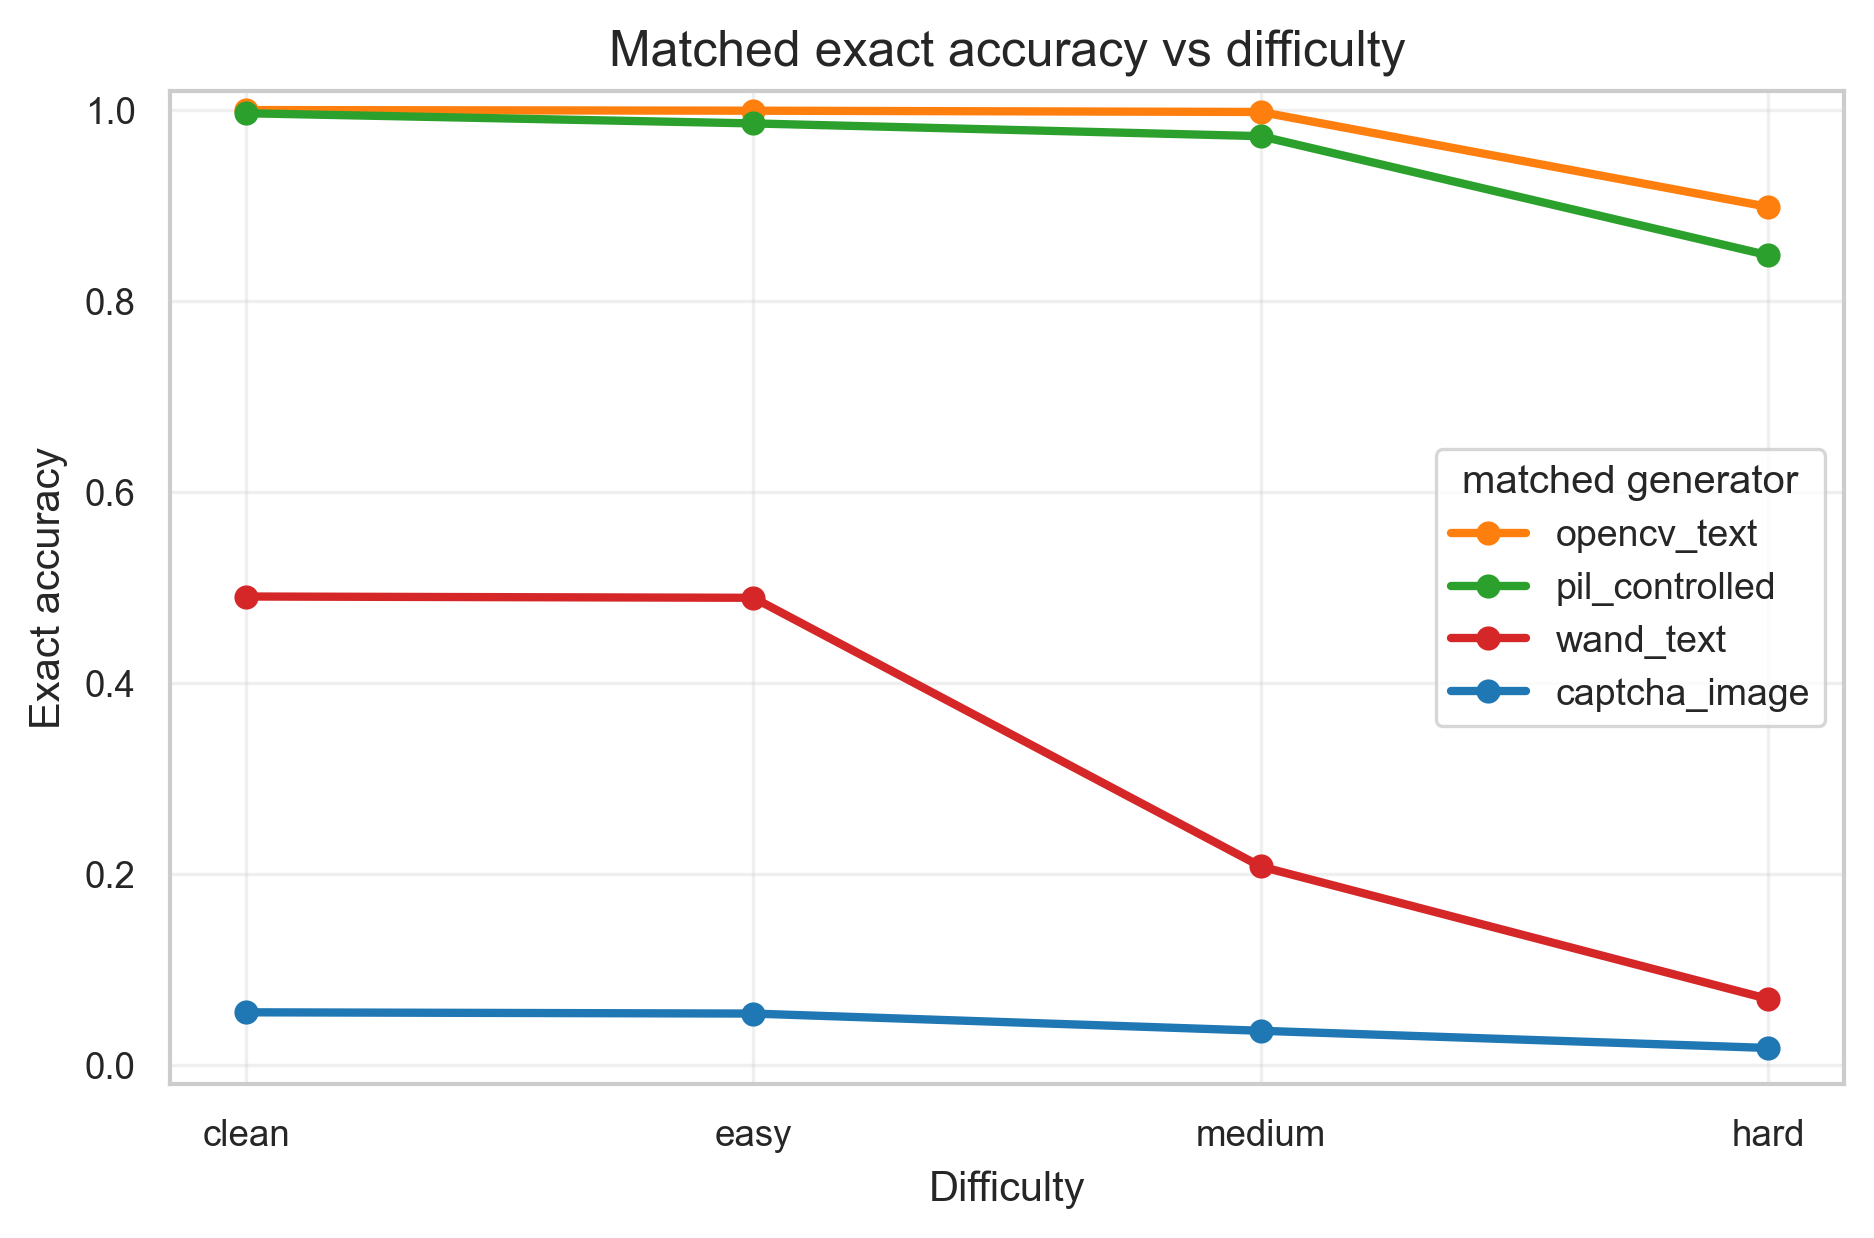
\includegraphics[width=\columnwidth]{figures/local_exact_accuracy_vs_difficulty.png}
    \caption{Exact-match accuracy versus difficulty under matched training across
    four generator families. \texttt{opencv\_text} degrades gracefully from
    100.00\% at clean to 89.87\% at hard; \texttt{pil\_controlled} from 99.67\%
    to 84.80\%; \texttt{wand\_text} from 49.07\% to 6.93\%; and
    \texttt{captcha\_image} remains below 5.53\% at all difficulty levels.
    The cross-generator range reflects rendering structure interacting with the fixed-slot architecture; it is not attributable to distortion intensity alone.}
    \label{fig:exact_acc_diff}
\end{figure}


The four matched-generator families fall into four distinct regimes under the
fixed-slot protocol. \texttt{opencv\_text} remains highly solvable across all
difficulty levels, reaching 100.00\% at clean and 89.87\% at hard with low ECE.
\texttt{pil\_controlled} also remains highly solvable, declining from 99.67\%
at clean to 84.80\% at hard. \texttt{wand\_text} has lower exact accuracy,
declining from 49.07\% at clean to 6.93\% at hard, together with poor
calibration. \texttt{captcha\_image} produces the lowest exact accuracy for this
fixed-slot preprocessing, from 5.53\% under clean to 1.80\% under hard.
These results support the narrower claim that generator choice interacts with
recognizer assumptions and can dominate measured benchmark performance.

\begin{table}[!htbp]
\centering
\caption{Wilson 95\% confidence intervals for primary exact-match accuracy
claims (1,500 test samples per condition).}
\label{tab:ci}
\resizebox{\columnwidth}{!}{%
\begin{tabular}{llcc}
\toprule
Generator & Difficulty & $A_{\mathrm{exact}}$ & 95\% CI \\
\midrule
\texttt{opencv\_text}    & Medium & 99.80\% & 99.41--99.93\% \\
\texttt{opencv\_text}    & Hard   & 89.87\% & 88.24--91.29\% \\
\texttt{pil\_controlled} & Medium & 97.27\% & 96.31--97.98\% \\
\texttt{pil\_controlled} & Hard   & 84.80\% & 82.89--86.53\% \\
\texttt{wand\_text}      & Medium & 20.80\% & 18.82--22.93\% \\
\texttt{captcha\_image}  & Medium & 3.60\%  & 2.77--4.67\% \\
\bottomrule
\end{tabular}
}
\end{table}

\FloatBarrier
\subsection{Cross-Generator Transfer Evaluation}
\label{sec:transfer}

Table~\ref{tab:transfer_full} and Figure~\ref{fig:transfer_matrix} present the
cross-generator exact accuracy matrix at medium difficulty.

\begin{table}[!htbp]
\centering
\caption{Cross-generator exact-match accuracy matrix at medium difficulty
(1,500 test samples per cell). Row = train generator; Column = test generator.
Diagonal = matched distribution. Off-diagonal = transfer. Transfer is
asymmetric and generally near-zero for \texttt{captcha\_image} (column~1)
and \texttt{wand\_text} (column~4).}
\label{tab:transfer_full}
\resizebox{\columnwidth}{!}{%
\begin{tabular}{lcccc}
\toprule
\textbf{Train}$\downarrow$ / \textbf{Test}$\rightarrow$
    & \texttt{captcha\_image}
    & \texttt{opencv\_text}
    & \texttt{pil\_controlled}
    & \texttt{wand\_text} \\
\midrule
\texttt{captcha\_image}  & \textbf{0.036} & 0.048 & 0.015 & 0.002 \\
\texttt{opencv\_text}    & 0.000 & \textbf{0.998} & 0.230 & 0.005 \\
\texttt{pil\_controlled} & 0.000 & 0.601 & \textbf{0.973} & 0.037 \\
\texttt{wand\_text}      & 0.000 & 0.233 & 0.619 & \textbf{0.208} \\
\bottomrule
\end{tabular}
}
\end{table}

\begin{figure}[!htbp]
    \centering
    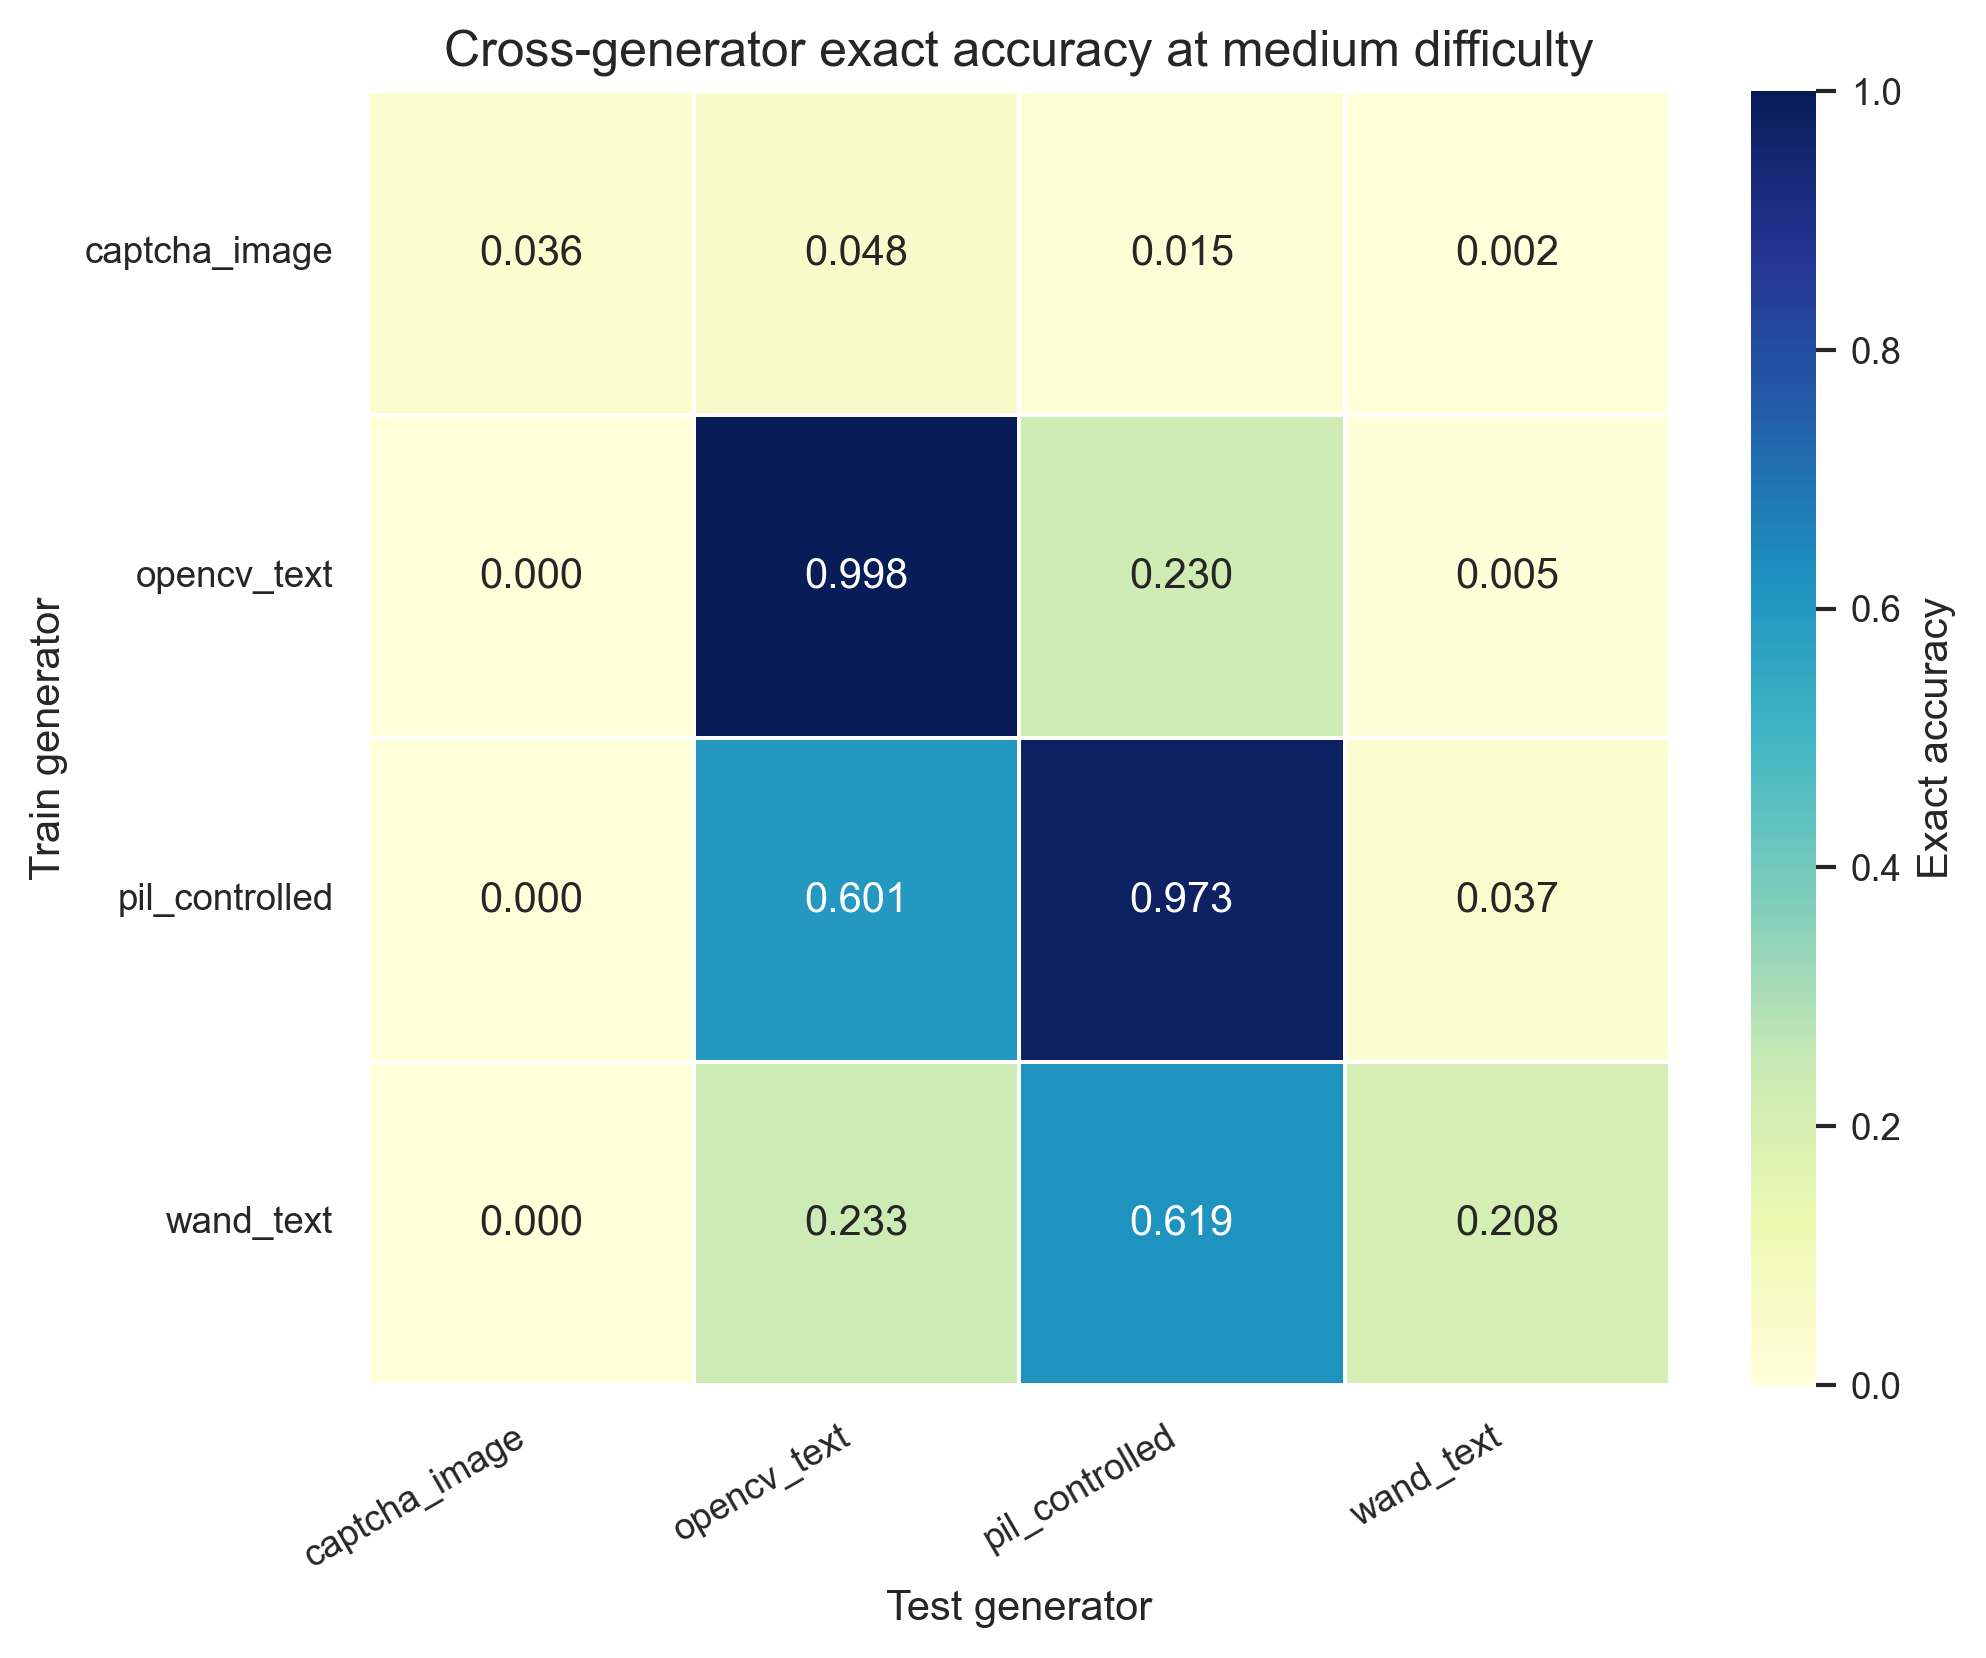
\includegraphics[width=\columnwidth]{figures/local_transfer_matrix.png}
    \caption{Heatmap of cross-generator exact-match accuracy at medium difficulty
    (1,500 test samples per cell). No model trained on any generator achieves
    non-trivial accuracy on \texttt{captcha\_image} (leftmost column).
    Transfer is strongly asymmetric: the \texttt{pil\_controlled}-trained model
    transfers to \texttt{opencv\_text} at 60.1\%, while the reverse is only
    23.0\%. \texttt{wand\_text} transfers to \texttt{pil\_controlled} at 61.9\%,
    making it surprisingly informative as a training source despite low
    matched-distribution accuracy.}
    \label{fig:transfer_matrix}
\end{figure}

Three findings stand out. First, no trained model achieves non-trivial
accuracy on \texttt{captcha\_image} beyond its own weak matched baseline,
confirming that this family occupies a visually isolated region for the
fixed-slot architecture. Second, transfer among the remaining generators is
strongly asymmetric rather than negligible: \texttt{pil\_controlled} transfers
to \texttt{opencv\_text} at 60.1\%, \texttt{wand\_text} transfers to
\texttt{pil\_controlled} at 61.9\%, and \texttt{wand\_text} transfers to
\texttt{opencv\_text} at 23.3\%. Third, high matched-distribution accuracy
does not imply broad transfer. Even the \texttt{opencv\_text}-trained model,
which reaches 99.8\% exact accuracy in-distribution, drops to 23.0\% on
\texttt{pil\_controlled} and 0.5\% on \texttt{wand\_text}. Multi-generator
testing is therefore necessary: a single-generator benchmark cannot support
general claims about CAPTCHA vulnerability.

In conclusion, the implications are clear --- benchmark performance on a local
generator should \emph{not} be used to infer general robustness of the model,
since it is likely to perform poorly on different generators. Multi-generator
testing is required to properly assess the solver's vulnerabilities.

\FloatBarrier
\subsection{Reliability Analysis}
\label{sec:reliability_results}

\textbf{Temperature Scaling and Calibration.}
Table~\ref{tab:tempscale} presents the results of post-hoc temperature scaling
procedure~\cite{guo2017calibration}. In our case, optimal temperatures differ
between models. For example, \texttt{opencv\_text} uses $T=0.677$,
\texttt{pil\_controlled} uses $T=0.739$, and \texttt{captcha\_image} uses
$T=1.156$. Temperature scaling decreases NLL in all four cases, but the change is small for the weak models (\texttt{wand\_text}: 0.986 to 0.986; \texttt{captcha\_image}: 1.948 to 1.932),
but it cannot save inaccurate generator types; it modifies confidence
and not the predicted results. 

\begin{table}[!htbp]
    \centering
    \caption{Temperature Scaling of Post-training Generator Models. The $T > 1$ ratio implies overconfidence, whereas $T < 1$ means underconfidence relative to empirical accuracy. The post-scaling NLL and validation accuracy $A_{\text{exact}}$ are provided for comparison; NLL decreases when scaling helps. The validation accuracies (0.999, 0.967, 0.244, 0.033) come from the held-out validation split, whereas Table~\ref{tab:matched_gen_full} reports full-scale medium-trained test values.}
    \label{tab:tempscale}
    \resizebox{\columnwidth}{!}{%
    \begin{tabular}{lcccc}
        \toprule
        Generator & $T$ & $\text{NLL}_{\text{before}}$ & $\text{NLL}_{\text{after}}$ & Val $A_{\text{exact}}$ \\
        \midrule
        \texttt{opencv\_text}    & 0.677 & 0.004 & 0.003 & 0.999 \\
        \texttt{pil\_controlled} & 0.739 & 0.022 & 0.020 & 0.967 \\
        \texttt{wand\_text}      & 0.975 & 0.986 & 0.986 & 0.244 \\
        \texttt{captcha\_image}  & 1.156 & 1.948 & 1.932 & 0.033 \\
        \bottomrule
    \end{tabular}
    }
\end{table}

Figure~\ref{fig:calibration} represents the relationship between ECE and difficulty level. It can be seen that both variables correlate, but not proportionally: \texttt{captcha\_image} with medium difficulty level demonstrates an exact accuracy of 3.60\%, along with ECE of 0.3520, whereas \texttt{pil\_controlled} with medium difficulty level provides 97.27\% of exact accuracy, with ECE being 0.0197. However, the \texttt{opencv\_text} generator with hard difficulty level shows 89.87\% exact accuracy and ECE of 0.0851, indicating that confidence
remains informative even at the boundary of the model's capability.

\begin{figure}[!htbp]
    \centering
    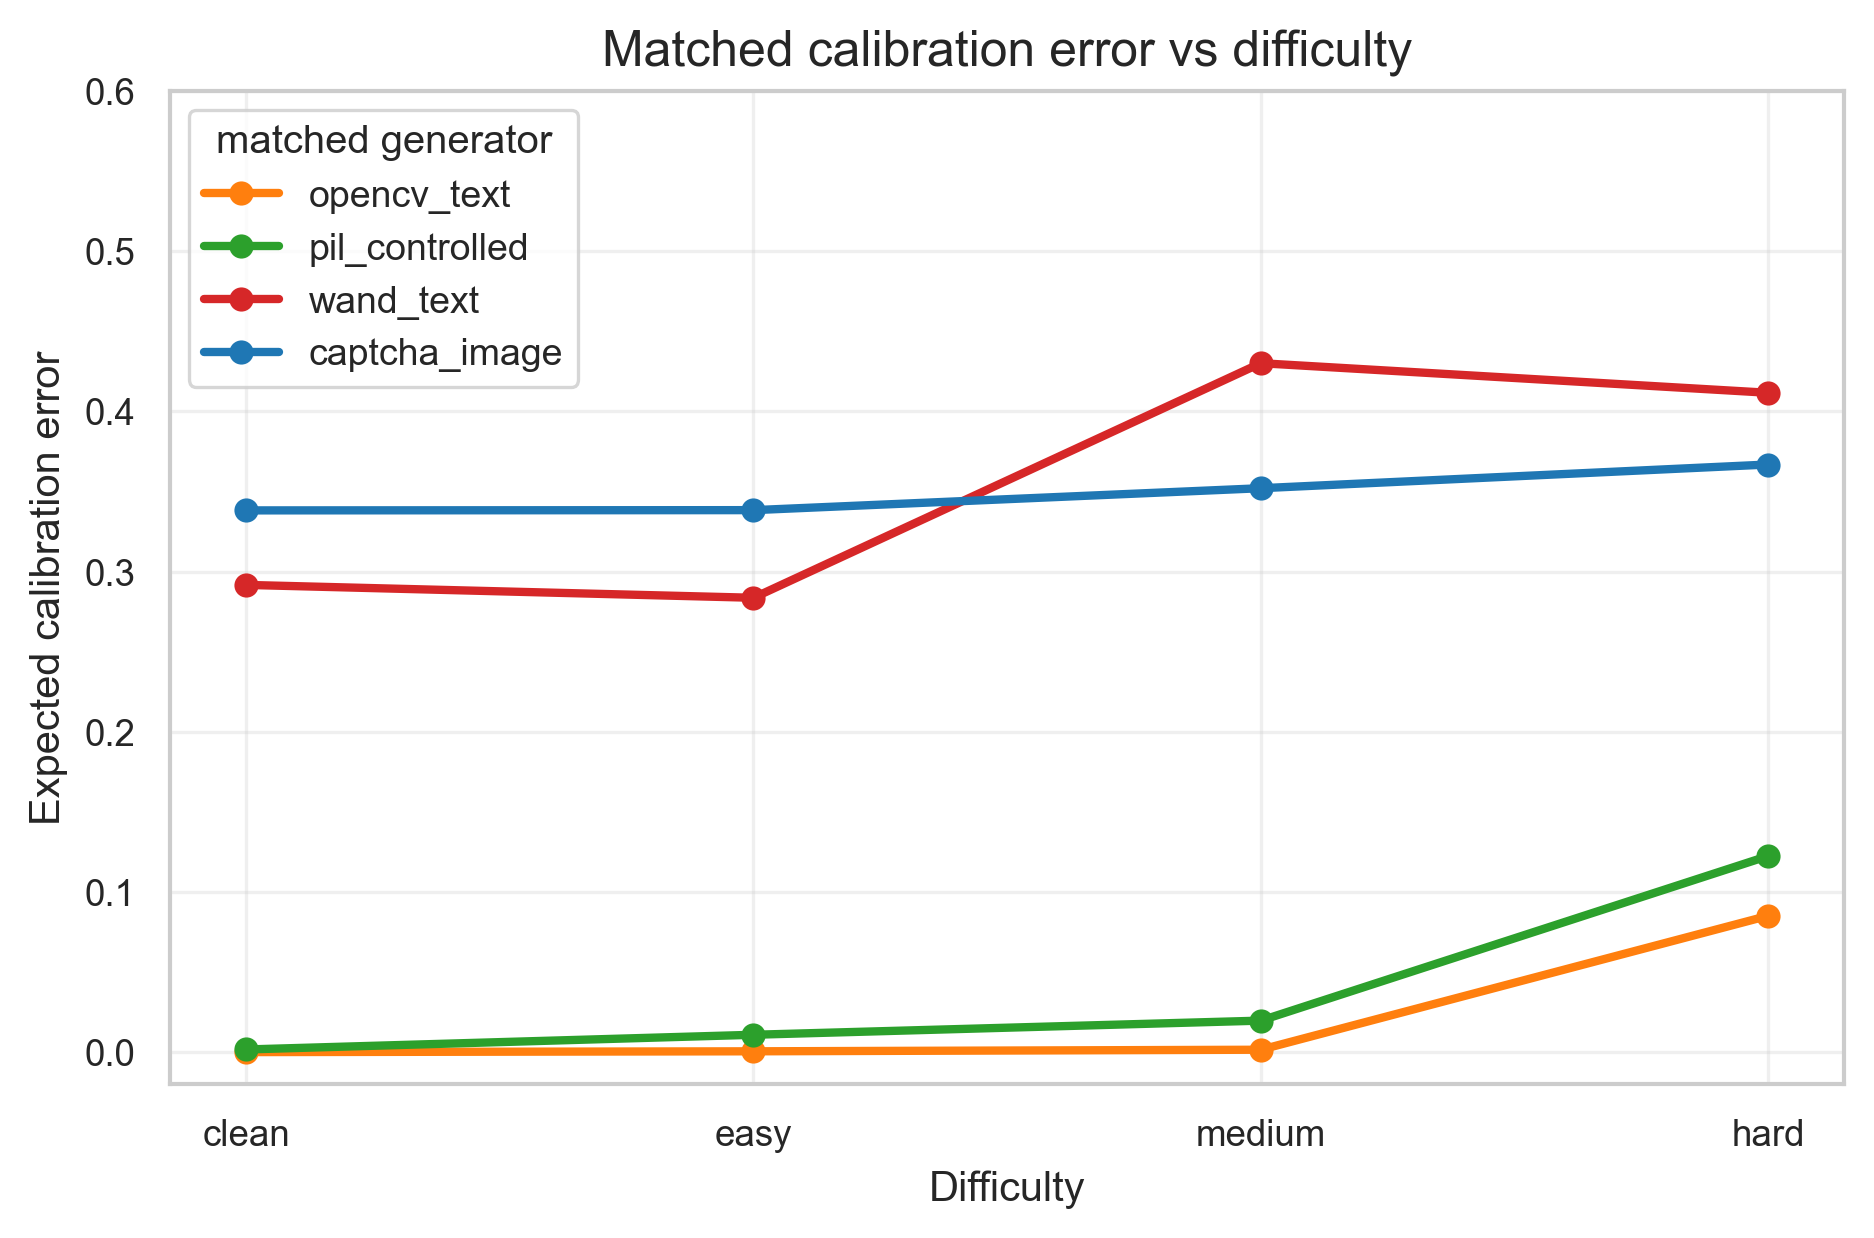
\includegraphics[width=\columnwidth]{figures/local_calibration_error_vs_difficulty.png}
    \caption{Expected calibration error (ECE) versus difficulty under matched
    training. Low ECE indicates well-aligned confidence and accuracy.
    \texttt{opencv\_text} maintains low ECE across all difficulty levels;
    \texttt{pil\_controlled} ECE rises steeply with difficulty; and
    \texttt{captcha\_image} models exhibit elevated ECE throughout, reflecting
    systematic overconfidence on structurally unsolvable inputs.}
    \label{fig:calibration}
\end{figure}

\textbf{Out-of-Distribution Detection}
Table~\ref{tab:ood} presents entropy-based AUROC for OOD detection~\cite{hendrycks2017baseline,liang2018enhancing}.
The entropy detector is directionally informative for some shifts: the model trained with \texttt{opencv\_text} attains an AUROC score of 0.9999 against
\texttt{captcha\_image}@medium due to low in-distribution entropy and higher OOD entropy. For \texttt{pil\_controlled}@medium, the model attains an AUROC score of 0.9983 against \texttt{captcha\_image}@medium, but a score of 0.7341 for \texttt{pil\_controlled}@hard. This lower AUROC is expected since difficult in-family samples preserve more of the training distribution's structure.
The \texttt{captcha\_image}-trained model has weaker cross-generator OOD discrimination, with AUROC values ranging from 0.3055 to 0.5852 across the medium cross-generator conditions. Values below 0.5 indicate that entropy is systematically lower on the designated OOD set; the label orientation was checked in the implementation by assigning ID=0 and OOD=1. We report entropy only; the cited energy-based method is discussed as related work, not as an evaluated score.

\begin{table}[!htbp]
    \centering
    \caption{Entropy-based OOD detection AUROC. Each row reports a trained
    model evaluated against an OOD condition. Higher AUROC indicates stronger
    discrimination between in-distribution and out-of-distribution inputs via
    sequence entropy.}
    \label{tab:ood}
    \resizebox{\columnwidth}{!}{%
    \begin{tabular}{llc}
        \toprule
        Train generator & OOD condition & AUROC \\
        \midrule
        \texttt{opencv\_text}    & \texttt{captcha\_image}@medium  & 0.9999 \\
        \texttt{opencv\_text}    & \texttt{wand\_text}@medium      & 0.9994 \\
        \texttt{opencv\_text}    & \texttt{pil\_controlled}@medium & 0.9882 \\
        \texttt{opencv\_text}    & \texttt{opencv\_text}@hard      & 0.7915 \\
        \midrule
        \texttt{pil\_controlled} & \texttt{captcha\_image}@medium  & 0.9983 \\
        \texttt{pil\_controlled} & \texttt{wand\_text}@medium      & 0.9884 \\
        \texttt{pil\_controlled} & \texttt{opencv\_text}@medium    & 0.8484 \\
        \texttt{pil\_controlled} & \texttt{pil\_controlled}@hard   & 0.7341 \\
        \midrule
        \texttt{captcha\_image}  & \texttt{opencv\_text}@medium    & 0.5852 \\
        \texttt{captcha\_image}  & \texttt{pil\_controlled}@medium & 0.4627 \\
        \texttt{captcha\_image}  & \texttt{wand\_text}@medium      & 0.3055 \\
        \texttt{captcha\_image}  & \texttt{captcha\_image}@hard    & 0.5116 \\
        \midrule
        \texttt{wand\_text}      & \texttt{captcha\_image}@medium  & 0.6517 \\
        \texttt{wand\_text}      & \texttt{opencv\_text}@medium    & 0.2666 \\
        \texttt{wand\_text}      & \texttt{pil\_controlled}@medium & 0.1293 \\
        \texttt{wand\_text}      & \texttt{wand\_text}@hard        & 0.7711 \\
        \bottomrule
    \end{tabular}
    }
\end{table}

\textbf{Abstention.}
The coverage versus selective accuracy abstention plot is depicted in
Figure~\ref{fig:abstention}. For \texttt{opencv\_text} and
\texttt{pil\_controlled}, confidence thresholding preserves high selective
accuracy at substantial coverage, showing that confidence remains informative
when the matched model is already strong. For \texttt{wand\_text}, selective
accuracy improves only by sacrificing much more coverage. For
\texttt{captcha\_image}, abstention does not rescue performance: the best
medium operating point above 50\% coverage reaches only 5.37\% selective
accuracy.

\begin{figure}[!htbp]
    \centering
    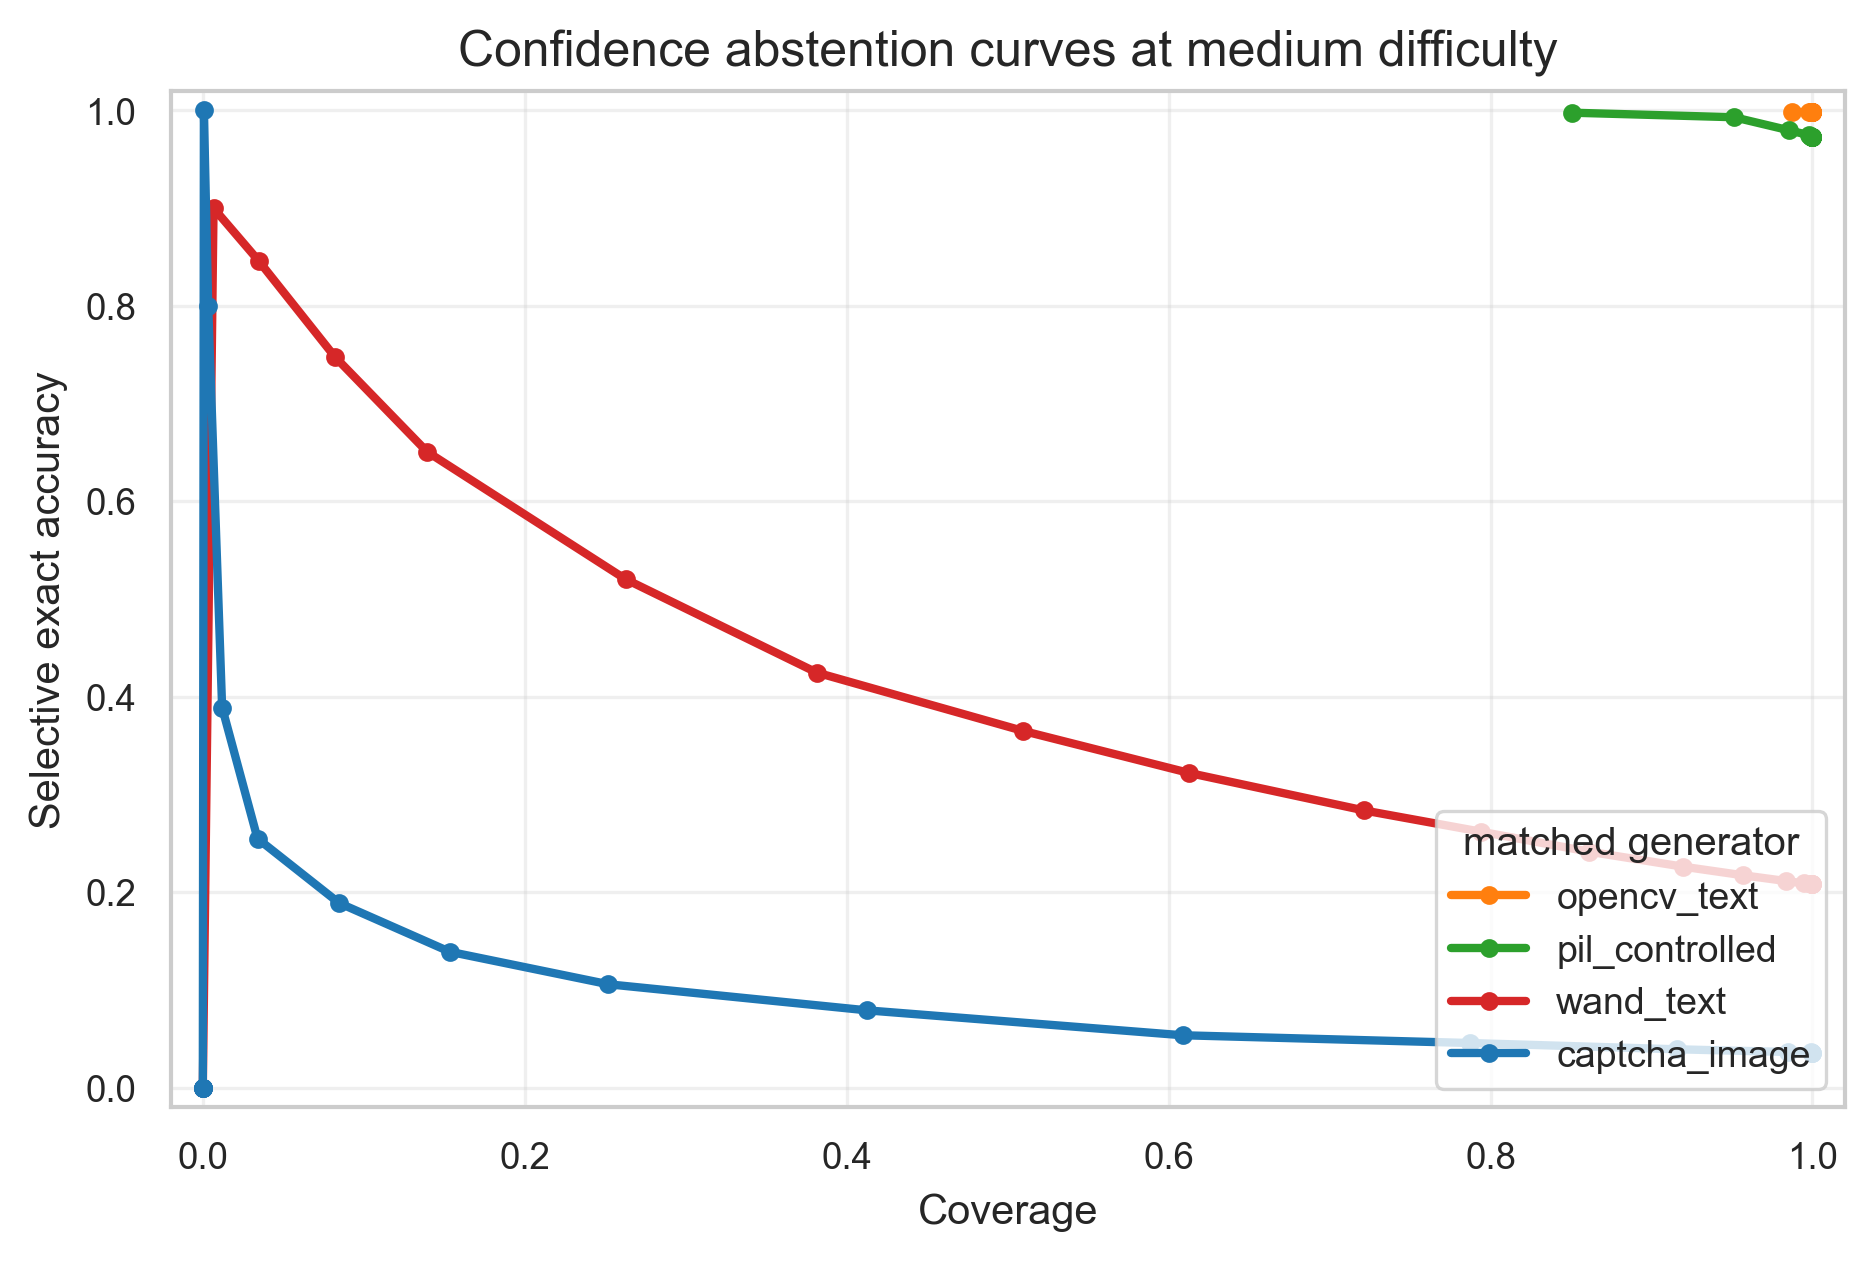
\includegraphics[width=\columnwidth]{figures/local_abstention_curves.png}
    \caption{Coverage vs.\ selective accuracy abstention curves across
    generator-difficulty conditions. Coverage is the fraction of predictions
    retained above a confidence threshold; selective accuracy is accuracy on
    retained predictions. Curves that rise steeply toward the upper-left
    indicate informative confidence scores. Flat curves indicate uniformly
    uninformative scores.}
    \label{fig:abstention}
\end{figure}

In combination, the results of the reliability analyses show that the ECE,
OOD AUROC, and abstention utilities vary with solver accuracy in a manner
that is nontrivial: the \emph{ordering} of the different generator families
by their calibration performance cannot simply be derived from their solve
rates alone. A generator that performs reasonably well on the task may have
severely mis-calibrated confidence estimates, while a highly accurate
solver can have good OOD discrimination ability and abstention ability.
These factors are invisible using solve rates only.


\FloatBarrier
\subsection{Failure Taxonomy}
\label{sec:taxonomy}

The errors associated with each incorrect prediction are classified according to error type in Table~\ref{tab:taxonomy} and Figure~\ref{fig:taxonomy}, based on the failure-taxonomy artifact. The rows pool the four trained models evaluated on each condition (6,000 predictions); correct predictions are excluded from the denominator. Because all models emit five positions, insertion and deletion are inoperative in this analysis; the taxonomy therefore provides information mainly about substitutions, transpositions, and repeated-character errors.

\begin{table}[!htbp]
\centering
\caption{Failure taxonomy: Percentage of each error type among incorrect
predictions, for each generator and difficulty level. Each row pools the
four trained models evaluated on that test condition (6,000 predictions);
correct predictions are excluded from the denominator. Insertion and
deletions are structurally zero because the fixed-slot decoder always emits
five characters. SUB = substitution; DEL
= deletion (predicted string is shorter than the original); INS = insertion
(predicted string is longer than the original); REP = repeat (all characters are predicted identically); TRN = transposition.}
\label{tab:taxonomy}
\resizebox{\columnwidth}{!}{%
\begin{tabular}{llccccc}
\toprule
Generator & Difficulty & SUB (\%) & DEL (\%) & INS (\%) & REP (\%) & TRN (\%) \\
\midrule
\texttt{pil\_controlled} & Clean  & 99.97 & 0.00 & 0.00 & 0.00 & 0.03 \\
\texttt{pil\_controlled} & Easy   & 99.97 & 0.00 & 0.00 & 0.00 & 0.03 \\
\texttt{pil\_controlled} & Medium & 99.91 & 0.00 & 0.00 & 0.03 & 0.06 \\
\texttt{pil\_controlled} & Hard   & 99.95 & 0.00 & 0.00 & 0.03 & 0.03 \\
\texttt{opencv\_text}    & Clean  & 100.00 & 0.00 & 0.00 & 0.00 & 0.00 \\
\texttt{opencv\_text}    & Easy   & 100.00 & 0.00 & 0.00 & 0.00 & 0.00 \\
\texttt{opencv\_text}    & Medium & 100.00 & 0.00 & 0.00 & 0.00 & 0.00 \\
\texttt{opencv\_text}    & Hard   & 100.00 & 0.00 & 0.00 & 0.00 & 0.00 \\
\texttt{captcha\_image}  & Clean  & 97.40 & 0.00 & 0.00 & 2.54 & 0.07 \\
\texttt{captcha\_image}  & Easy   & 98.39 & 0.00 & 0.00 & 1.57 & 0.03 \\
\texttt{captcha\_image}  & Medium & 99.08 & 0.00 & 0.00 & 0.86 & 0.07 \\
\texttt{captcha\_image}  & Hard   & 98.38 & 0.00 & 0.00 & 1.61 & 0.02 \\
\texttt{wand\_text}      & Clean  & 99.90 & 0.00 & 0.00 & 0.08 & 0.02 \\
\texttt{wand\_text}      & Easy   & 99.48 & 0.00 & 0.00 & 0.46 & 0.06 \\
\texttt{wand\_text}      & Medium & 95.50 & 0.00 & 0.00 & 4.46 & 0.04 \\
\texttt{wand\_text}      & Hard   & 92.46 & 0.00 & 0.00 & 7.51 & 0.03 \\
\bottomrule
\end{tabular}
}
\end{table}

\begin{figure}[!htbp]
    \centering
    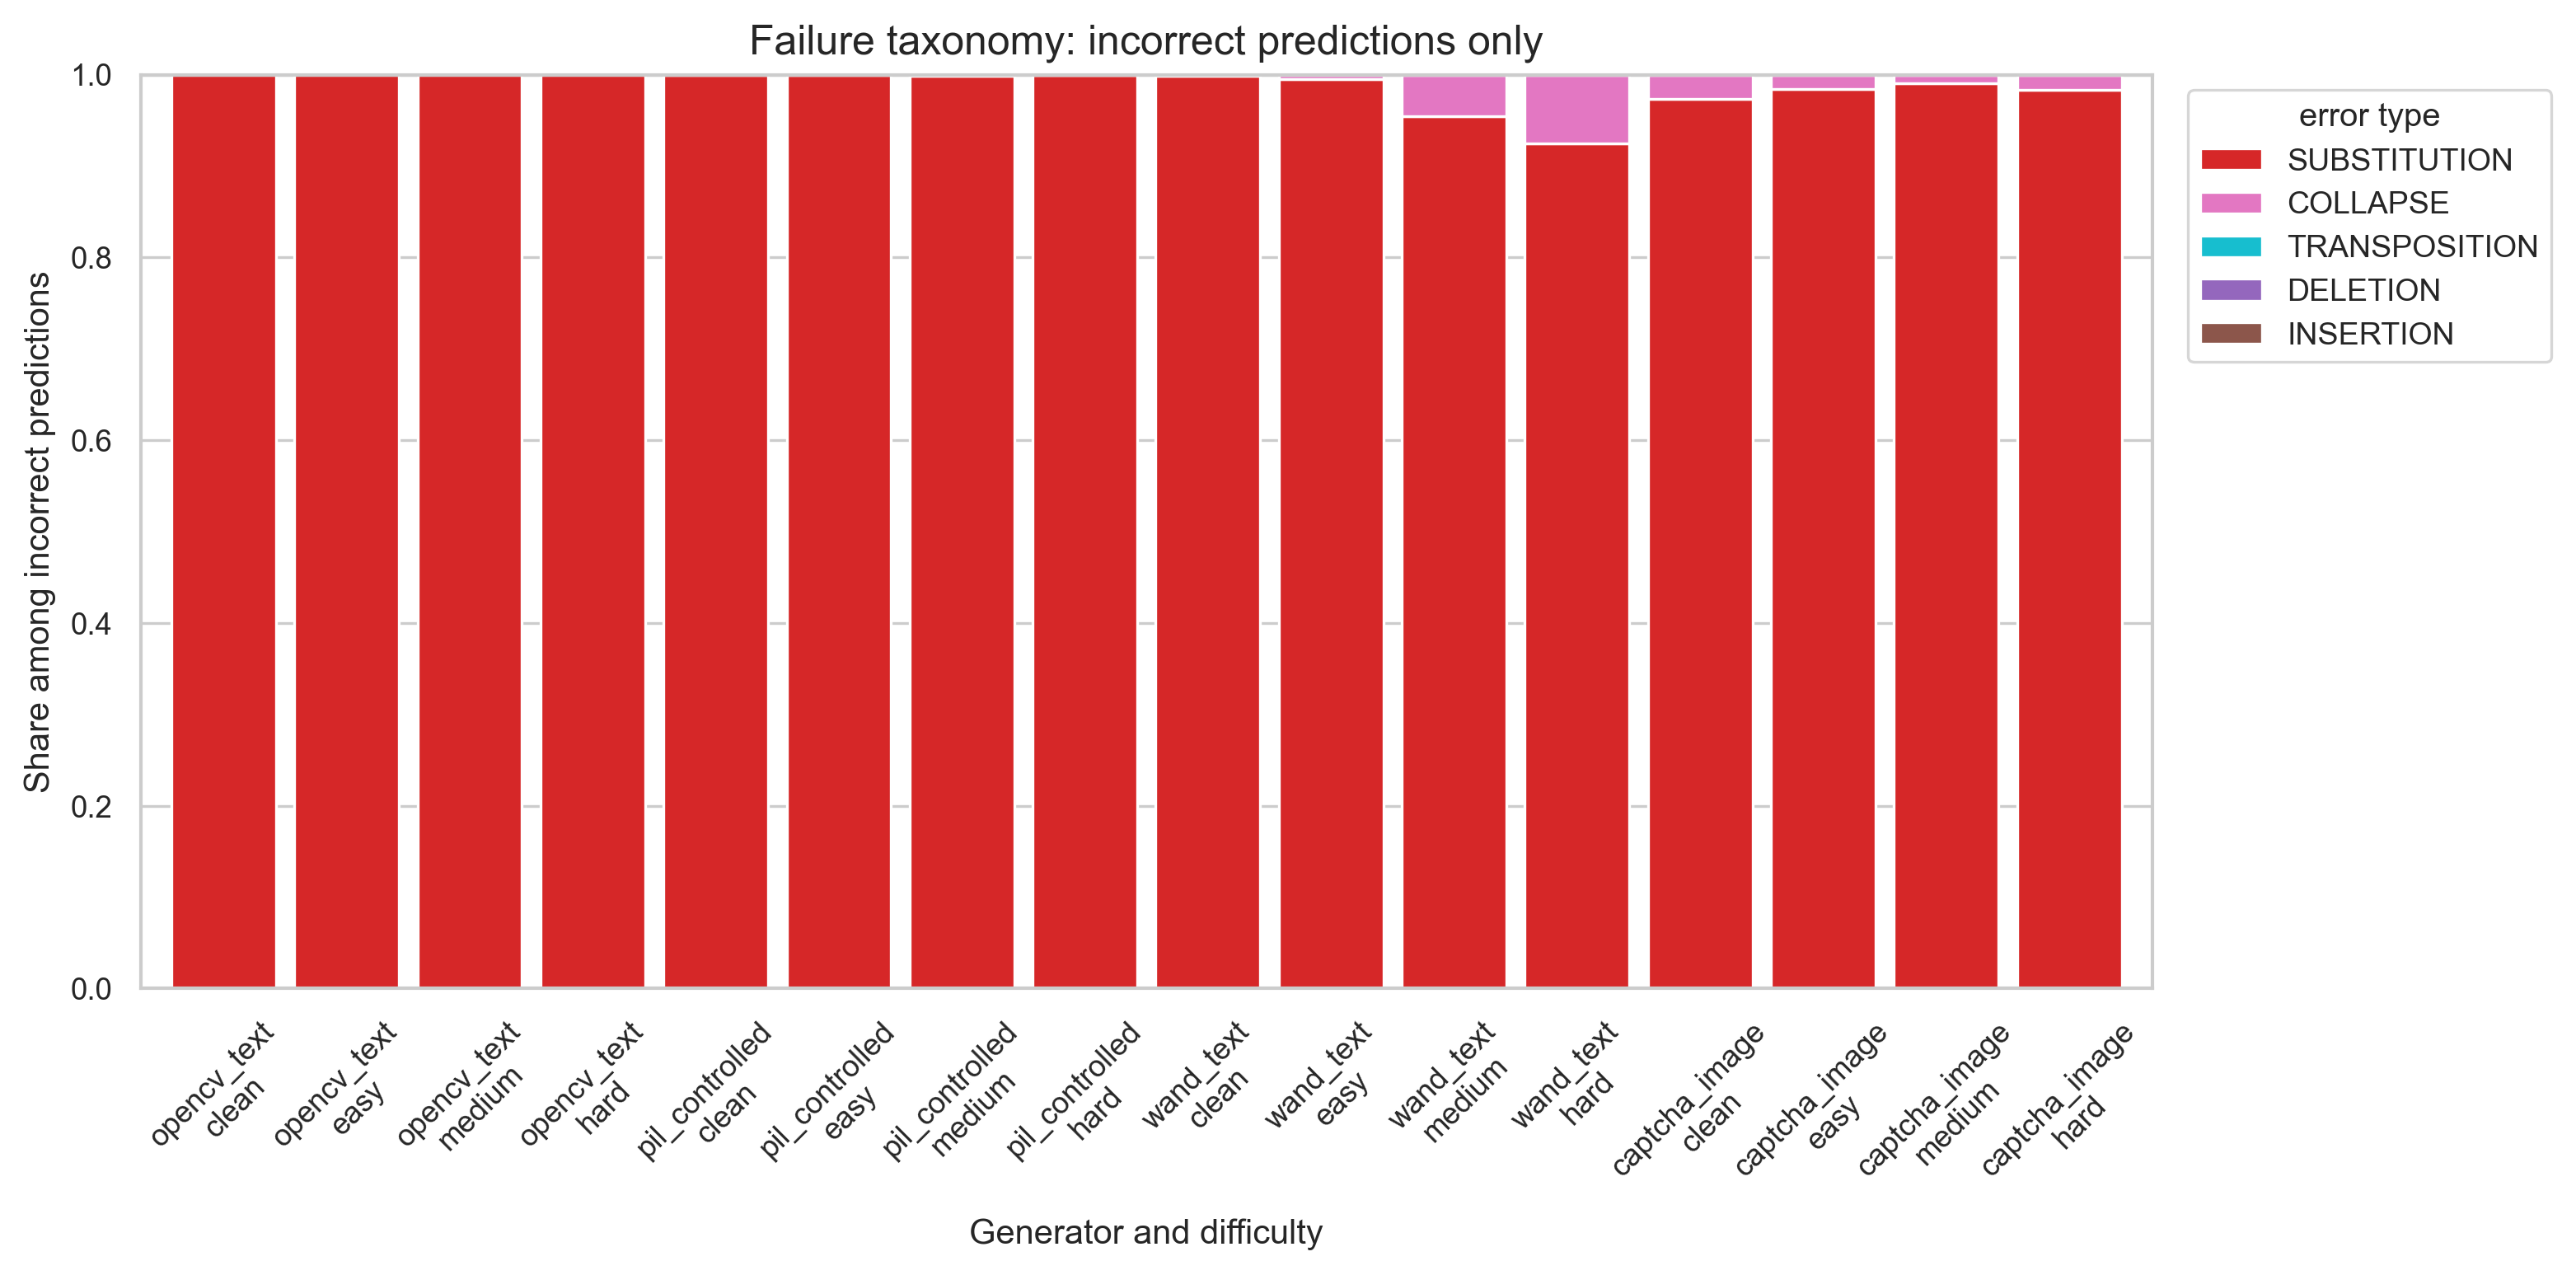
\includegraphics[width=\columnwidth]{figures/failure_taxonomy.png}
    \caption{Failure taxonomy based on incorrect predictions made by generator
    and task difficulty. Substitution is predominant in all groups,
    while repeated-character errors occur more often for difficult \texttt{wand\_text} and 
    \texttt{captcha\_image} tasks.}
    \label{fig:taxonomy}
\end{figure}
\FloatBarrier
\subsection{Vulnerability Scorecard (V-Score)}
\label{sec:vscore}

Substitutions account for the vast majority of failure cases out of all
96,000 predictions made, with 70,107 substitutions against 1,110 repeated-character errors and 24 transpositions. There are no insertions or deletions because the fixed-slot decoder produces exactly five characters. We call the repeated-character category ``repeat'' below to avoid confusing it with benchmark collapse.


Table~\ref{tab:vscore} presents the V-Score for each generator--difficulty
condition evaluated in this study. We use the formulation:
\begin{equation}
\label{eq:vscore}
R = w_1 A_{\mathrm{exact}} + w_2 (1 - \mathrm{ECE}) - w_3 H,
\end{equation}
where $H$ is the normalized average prediction entropy defined above. Given the default weights
$w_1=0.4$, $w_2=0.2$, and $w_3=0.2$, a high V-Score records stronger solver
evidence: high accuracy, good calibration, and low uncertainty. It is a
summary of these measurements, not a deployment-level vulnerability estimate.

\begin{table}[!htbp]
\centering
\caption{V-Score vulnerability scorecard across all generator--difficulty
conditions. Scores closer to the attainable upper bound 0.6 indicate strong
solver evidence under this formulation; scores near 0 indicate weak evidence.
Because $w_1+w_2=0.6$ and the remaining terms are non-positive, 1.0 is not
attainable. The ordering in this table agrees with exact accuracy; the score
adds calibration and entropy context without producing a ranking reversal.}
\label{tab:vscore}
\resizebox{\columnwidth}{!}{%
\begin{tabular}{llcccc}
\toprule
Generator & Difficulty & $A_{\mathrm{exact}}$ & ECE & Avg. entropy & V-Score \\
\midrule
\texttt{opencv\_text}    & Clean  & 1.0000 & 0.0001 & 0.0001 & 0.6000 \\
\texttt{opencv\_text}    & Easy   & 0.9993 & 0.0006 & 0.0002 & 0.5996 \\
\texttt{opencv\_text}    & Medium & 0.9980 & 0.0015 & 0.0007 & 0.5988 \\
\texttt{pil\_controlled} & Clean  & 0.9967 & 0.0017 & 0.0018 & 0.5980 \\
\texttt{pil\_controlled} & Easy   & 0.9860 & 0.0109 & 0.0026 & 0.5917 \\
\texttt{pil\_controlled} & Medium & 0.9727 & 0.0197 & 0.0060 & 0.5839 \\
\texttt{opencv\_text}    & Hard   & 0.8987 & 0.0851 & 0.0116 & 0.5401 \\
\texttt{pil\_controlled} & Hard   & 0.8480 & 0.1224 & 0.0208 & 0.5105 \\
\texttt{wand\_text}      & Clean  & 0.4907 & 0.2917 & 0.1697 & 0.3040 \\
\texttt{wand\_text}      & Easy   & 0.4893 & 0.2836 & 0.1776 & 0.3035 \\
\texttt{wand\_text}      & Medium & 0.2080 & 0.4301 & 0.2900 & 0.1392 \\
\texttt{wand\_text}      & Hard   & 0.0693 & 0.4116 & 0.4428 & 0.0569 \\
\texttt{captcha\_image}  & Clean  & 0.0553 & 0.3382 & 0.5532 & 0.0439 \\
\texttt{captcha\_image}  & Easy   & 0.0540 & 0.3383 & 0.5541 & 0.0431 \\
\texttt{captcha\_image}  & Medium & 0.0360 & 0.3520 & 0.5561 & 0.0328 \\
\texttt{captcha\_image}  & Hard   & 0.0180 & 0.3668 & 0.5596 & 0.0219 \\
\bottomrule
\end{tabular}
}
\end{table}

\begin{figure}[!htbp]
    \centering
    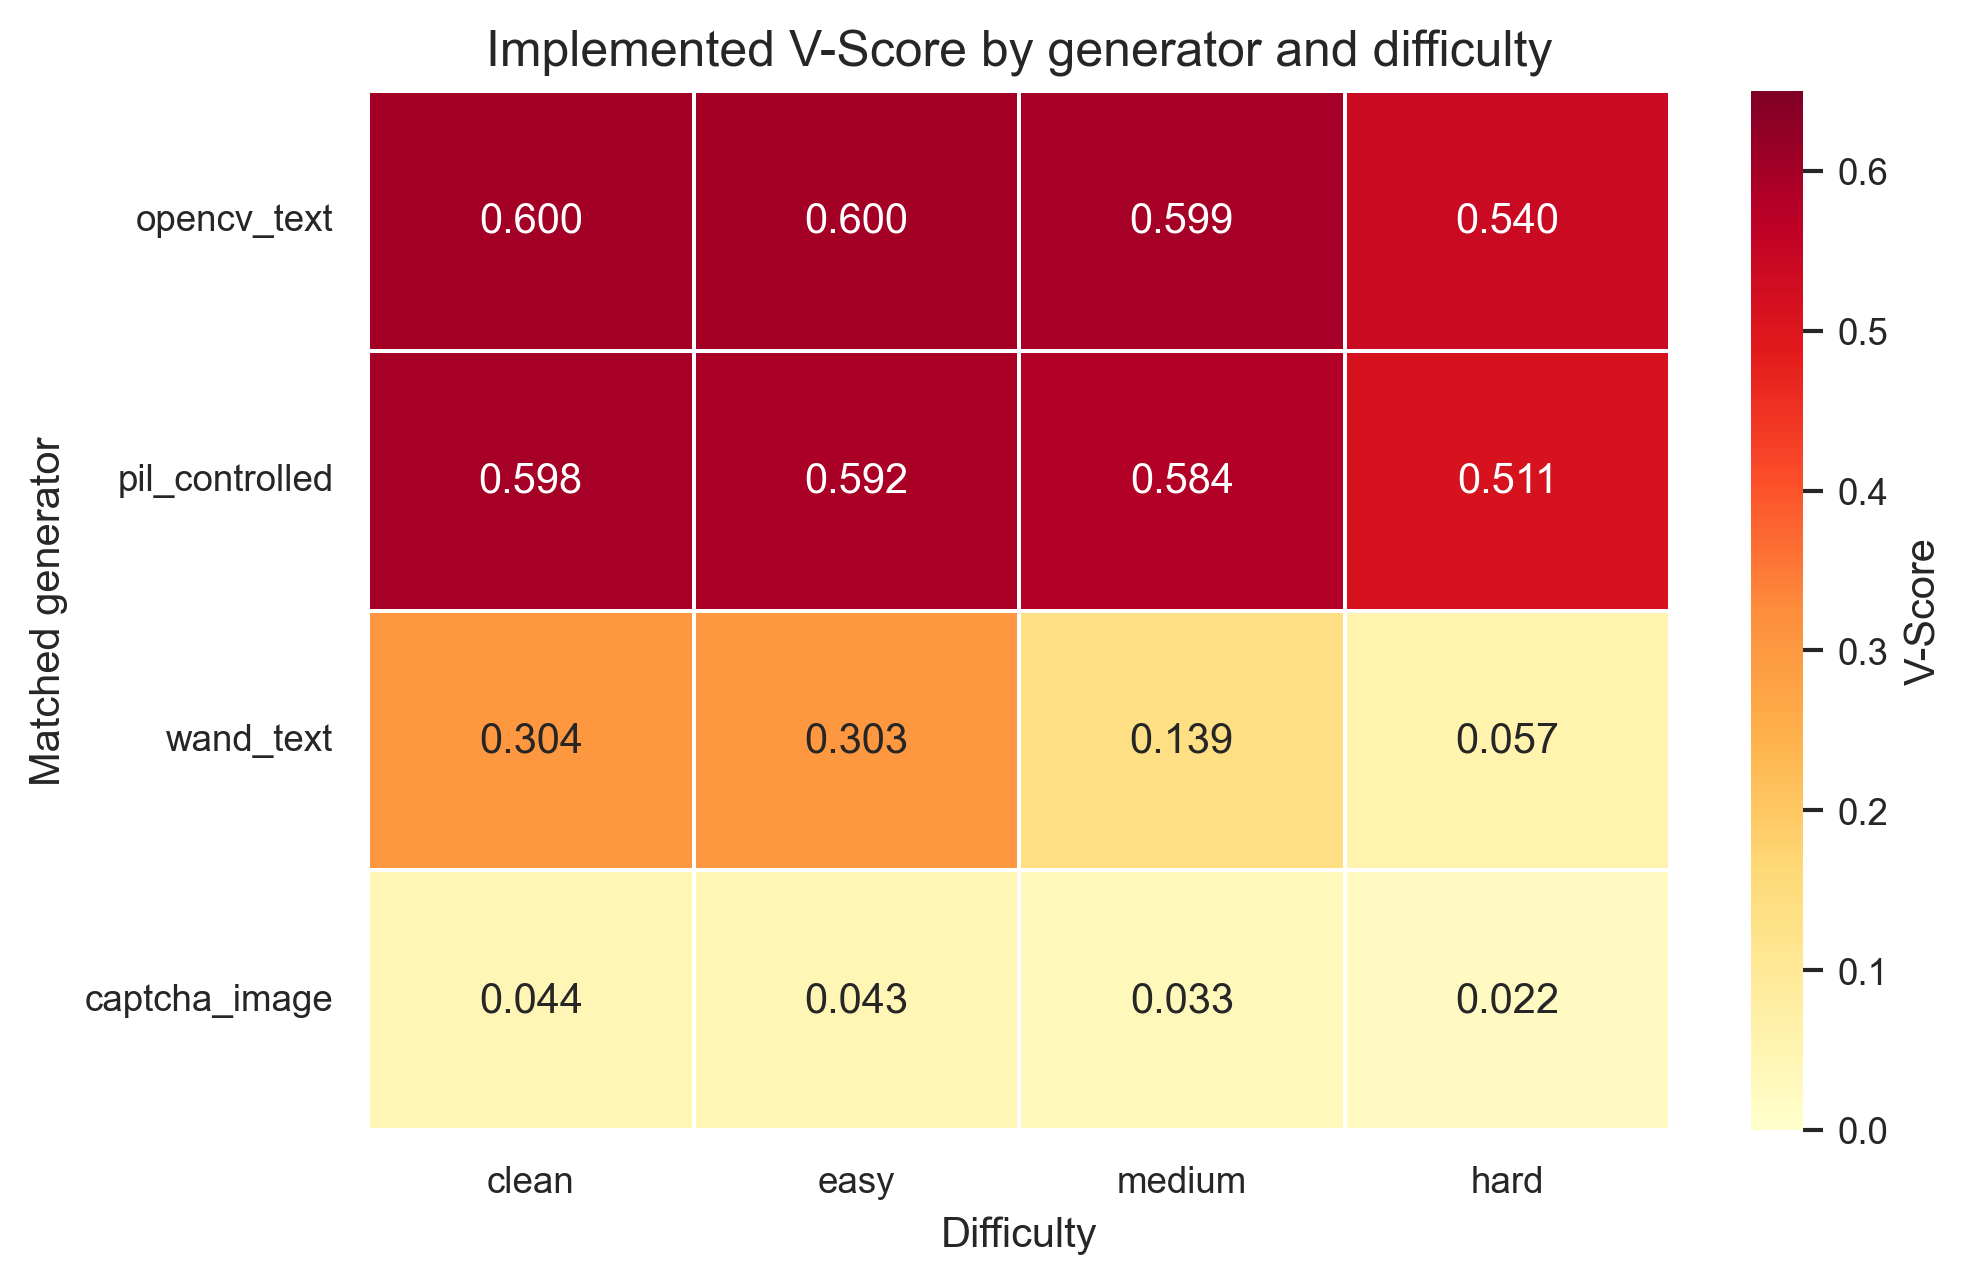
\includegraphics[width=\columnwidth]{figures/vscore_heatmap.png}
    \caption{Implemented V-Score heatmap for matched generator--difficulty
    conditions. Higher values indicate stronger solver evidence under the
    implemented score combining exact accuracy, calibration, and prediction
    entropy.}
    \label{fig:vscore_heatmap}
\end{figure}

\textbf{Key result:} The V-Score is a bounded reliability summary, not a
new ordering in these data. Recomputing it over all sixteen matched
conditions gives the same ordering as exact accuracy (Spearman $\rho=1.00$). For example, \texttt{opencv\_text}@hard achieves 89.87\% exact accuracy
with ECE below 0.09 and entropy near 0.01, whereas
\texttt{captcha\_image}@medium reaches 3.60\% with ECE above 0.35 and
entropy above 0.55. The score records this reliability difference, but the
reported table does not support a ranking reversal. The corresponding classifier cannot
serve any purpose in practice: it neither solves CAPTCHA problems nor
provides a low-uncertainty basis for decisions.
This is the type of situation that the V-Score is meant to detect.

\textbf{Sensitivity analysis.} Table~\ref{tab:vscore_sensitivity} shows the top five rows for five illustrative weight configurations. The underlying sensitivity artifact evaluates all sixteen matched generator--difficulty rows under each of the five explicitly listed weight configurations; lower-scoring rows were retained rather than omitted from the computation. OOD AUROC is reported separately and is not a V-Score term. Notably, the relative ranking of
\texttt{opencv\_text} (most vulnerable to attacks) and \texttt{captcha\_image}
(least vulnerable according to accuracy but also least reliable) remains
unchanged across the all-16-condition sensitivity analysis, although this
stability is expected because accuracy dominates the current monotone table.
We therefore present V-Score as a descriptive scorecard and do not claim that
these weights are theoretically optimal.

\begin{table}[!htbp]
\centering
\caption{Sensitivity analysis of the V-Score rankings for the top five generator--difficulty
configurations, as specified by the default ranking. The columns present V-Score values under the five explicitly listed weight configurations (default $(0.4,0.2,0.2)$, accuracy-only $(1,0,0)$, calibration-heavy $(0,0.8,0.2)$, entropy-heavy $(0,0.2,0.8)$, and equal-weight $(1/3,1/3,1/3)$), calculated using the provided implementation.}
\label{tab:vscore_sensitivity}
\resizebox{\columnwidth}{!}{%
\begin{tabular}{lccccc}
\toprule
Condition & Default & Accuracy-only & Calibration-heavy & Entropy-heavy & Equal-weight \\
\midrule
\texttt{opencv\_text}@clean    & 0.6000 & 1.0000 & 0.7999 & 0.1999 & 0.6666 \\
\texttt{opencv\_text}@easy     & 0.5996 & 0.9993 & 0.7995 & 0.1998 & 0.6662 \\
\texttt{opencv\_text}@medium   & 0.5988 & 0.9980 & 0.7986 & 0.1991 & 0.6653 \\
\texttt{pil\_controlled}@clean & 0.5980 & 0.9967 & 0.7983 & 0.1982 & 0.6644 \\
\texttt{pil\_controlled}@easy  & 0.5917 & 0.9860 & 0.7908 & 0.1957 & 0.6575 \\
\bottomrule
\end{tabular}
}
\end{table}

\FloatBarrier
% =============================================================
\section{Toward Reliability-Aware Evaluation}
\label{sec:architecture}
% =============================================================

The elements of reliability outlined above---calibration, out-of-distribution
detection, and abstention---have been empirically implemented and verified
through the local cross-generator benchmarking extension detailed in
Section~\ref{sec:local_extension}. This discussion addresses the design logic and
theory behind their implementation; the empirical results are found in
Section~\ref{sec:local_extension}. The core result stated in Section~\ref{sec:results} above represents the optimal case. In order to perform an exhaustive analysis of a model's vulnerabilities, it is necessary to consider harder cases -- when the accuracy of the model degrades significantly. Which cases will it happen, why and how confident it will be when it makes mistakes -- these questions cannot be answered solely based on the exact accuracy value.

We present a hierarchical structure with the generator, perception, reasoning and reliability layers, depicted in Fig. \ref{fig:architecture}, and address the following five aspects.

\subsection{Generator Layer: Auditable Difficulty}

To evaluate the performance of the generator under controlled synthetic conditions, it is necessary to parameterize its behavior in a way that would allow us to audit this process, i.e., trace all the steps taken by the generator to create a particular image. Specifically, the latter should come with a metadata annotation indicating exactly what set of parameters was used. As such, the current corrected PIL-based implementation of rendering covers only the case of clean images, which allows running controlled ablation studies of various distortions.

\subsection{Perception Layer: Stronger Backbone}

In order to run experiments with robustness in addition to the baseline one, the simple visual representation of the convolutional encoder can be changed into something that would allow more robust learning of features in the presence of blurring, rotations, and clutter. It could be a recent modern convolutional network~\cite{liu2022convnext} or an ensemble of convolutional layers and transformers~\cite{dosovitskiy2021vit}. Since the CAPTCHA-X framework is designed in a modular manner, it is straightforward to perform an experiment substituting backbone with another one.

\subsection{Reasoning Layer: CTC and Attention Decoding}

As for the text decoder, we suggest implementing a two-stage model consisting of CTC alignment~\cite{graves2006ctc} and attention decoding~\cite{vaswani2017attention}. For future multimodal tasks (image selection, semantic matching), the perception part may pass the image representation to an attention mechanism which would analyze different regions within the image to make decisions.

\subsection{Reliability Layer: Beyond Solve Rate}

Finally, here lies the essence of assessment itself, and the capabilities we should consider include:

\textbf{Calibration.} Temperature scaling of the model~\cite{guo2017calibration,naeini2015obtaining}
ensures that prediction confidence corresponds to accuracy. This was shown in
Section~\ref{sec:reliability_results}, where the optimal temperature ranges from
0.677 (\texttt{opencv\_text}, highly accurate and well-calibrated) to 1.156
(\texttt{captcha\_image}, overconfident and structurally mismatched).
Consequently, the confidence of a well-calibrated
model can serve as an informative feature for the vulnerability scorecard.

\textbf{Out-of-Distribution Detection.} Softmax entropy~\cite{hendrycks2017baseline,liang2018enhancing} or deeper energy scores~\cite{liu2020energy} detect when the input is out of the training distribution. This is directly relevant to CAPTCHA assessments since a good CAPTCHA solver should exhibit high uncertainty for an out-of-training-distribution image.

\textbf{Failure Taxonomy.} Failure classification into substitutions,
transpositions, and repeated-character outputs provides insight beyond
accuracy. Insertions and deletions are structurally inoperative here because
the decoder always emits five positions; we therefore do not interpret their
zero rates as evidence about general sequence recognizers.

\textbf{Abstention Policies.} An OOD-solver that abstains from solving on certain examples instead of guessing is more helpful for an attacker in the red-team analysis than a model that produces an answer anyway. The coverage-accuracy relationship defines the security surface at the system-level.

Combining these aspects together, the implemented vulnerability score used in
Section~\ref{sec:vscore} follows Equation~\ref{eq:vscore},
where $H$ is average prediction entropy. Broader scorecard variants can add
OOD and coverage terms, but the reported V-Score in this paper uses the
implemented reduced formulation above.

\subsection{Research Layer: Scorecards and Sweeps}

Finally, all these aspects can be rolled into an automated analysis report: solve-rates per difficulty, failure taxonomies, calibration graphs, OOD rejection rates, and human-machine accuracy gaps. If a family of CAPTCHAs scores well on the entire scorecard---high accuracy even for a high difficulty, perfect calibration, OOD robustness, and small human-machine gap---it can be considered more robust under the evaluated synthetic conditions. A clean solve rate should therefore be reported together with calibration and uncertainty, rather than interpreted as a deployment-level security claim.
% =============================================================
\section{Limitations and Scope Boundaries}

The following scope limitations have been consciously chosen:

\begin{itemize}
    \item \textbf{Only synthetic data.} All 160,000 images are locally synthesized. The results describe benchmark behavior under controlled synthetic rendering and do not establish breakability of deployed CAPTCHA services. 
    No live CAPTCHA service is utilized at any point. The central claim of the paper is that 
    synthetic benchmarks are already unreliable; applying the same to live services without fixing 
    the issue of synthetic reliability first would exacerbate the problem rather than solve it.
    Real-world transferability will be addressed explicitly later.

    \item \textbf{Fixed-slot architecture.} Fixed-slot architecture requires knowledge of the length
    of the string and regularity within positions. It is useful for isolating the
    collapse-like interaction studied here. The reduced CRNN pilot below tests
    whether the qualitative pattern survives a second architecture family; a
    full-scale CRNN/ViT/ConvNeXt comparison remains future work.

    \item \textbf{Single seed.} The full-scale matrix uses seed 17. We additionally ran a five-seed reduced pilot (seeds 17, 42, 99, 123, 256; 3,000 images per generator-condition and 450 test examples per cell). On the matched medium diagonal, exact accuracy was $0.941\pm0.047$ for \texttt{opencv\_text} and $0.549\pm0.171$ for \texttt{pil\_controlled}; the corresponding clean/easy/hard means were $0.988\pm0.016$/$0.992\pm0.009$/$0.716\pm0.094$ and $0.700\pm0.159$/$0.663\pm0.196$/$0.339\pm0.123$. The Wilson intervals in Table~\ref{tab:ci} quantify test-set sampling only; the pilot standard deviations quantify seed variation for the reduced protocol and are not uncertainty intervals for the full-scale run.

    \item \textbf{Human baseline not yet collected.} A human study harness
    (stimulus server, response logger, IRB scaffold) is implemented. No
    participant data has been collected. Human accuracy is therefore not reported. We retain $\tau_{\mathrm{human}}=0.85$ only as a literature-derived sensitivity anchor, not as an observed human baseline. Under the strict $>$ definition, the matched full-scale cells above 0.85 are 7 at $\tau=0.85$ (all four \texttt{opencv\_text} levels and \texttt{pil\_controlled} clean/easy/medium), 8 at $\tau=0.75$, 6 at $\tau=0.90$, and 6 at $\tau=0.95$.
    The pilot study is the most immediate next step.

    \item \textbf{Architecture pilot.}
    A reduced CRNN pilot is now included as an architecture-family check. It uses 1,000/200/200 examples per generator for train/validation/test and three epochs; because it is deliberately smaller than the headline experiment, we do not treat it as a replacement for a full-scale architecture comparison.
\end{itemize}
% =============================================================
\section{Reproducibility}
% =============================================================

Reproducibility is a first-class contribution of this work. The revision package includes the manuscript source, configuration files, audit reports, pilot summaries, and scripts needed to reproduce the reported analyses. The anonymized review artifact repository is available at \href{https://github.com/lakshitsachdeva/captcha-x-review-2026}{the review repository}.

The benchmark is designed so that a second evaluator can regenerate the data distribution from the configuration alone and verify the reported numbers. The generator, preprocessing, training, and evaluation scripts are all version-controlled and exercised in a documented demo. In sharp contrast, many previous CAPTCHA papers lacked the proper specification of the parameters of their generators, fonts used, and splitting schemes.
% =============================================================
\section{Responsible Use}
% =============================================================
The study is intended for defensive benchmark auditing. All experiments are
offline and use locally synthesized images; no live service is contacted and no
bypass claim is made. The reported best-case results therefore describe a failure
mode of a controlled benchmark under a specified generator, training procedure,
and evaluation set, rather than a claim about deployed CAPTCHA systems.

% =============================================================
\section{Conclusion}
This paper argues, and shows through experiments, that results on CAPTCHA benchmarks depend as much on the choice of generator as they do on the model itself. The argument is based on four main observations.
First, the original pipeline was reported to produce artifacts in its so-called
``clean'' setting, and the corrected renderer passes the available audit. The
original pre-repair image archive is unavailable, so we present this as a
provenance finding and do not claim a reproducible quantitative reconstruction. This is not just a one-off implementation issue---it points to a broader gap in how benchmark integrity is typically checked in CAPTCHA research, where generator settings are often taken at face value without inspecting the actual outputs.
Second, we evaluated 96,000 predictions across four generators and four difficulty levels. In the matched full-scale sweep, accuracy ranged from 100.00\% (\texttt{opencv\_text}@clean) to 1.80\% (\texttt{captcha\_image}@hard). This 55$\times$ cross-condition range includes different difficulty levels; the difficulty-matched medium range is 99.80\% versus 3.60\%, or 27.7$\times$. These spreads reflect an interaction between rendering structure and the fixed-slot architecture, not rendering structure alone. The fixed-slot collapse-like behavior is consistent with the operational
indicators in Proposition~\ref{thm:collapse}; the low scores on
\texttt{captcha\_image} and \texttt{wand\_text} should be read as architecture--renderer
interactions rather than generator-intrinsic difficulty.
Third, accuracy by itself turns out to be a weak proxy for security. Using the V-Score breakdown, we observe that some generators with near-zero exact-match accuracy still show poor calibration and high prediction entropy. That combination is unstable from a security perspective. By contrast, a model achieving 89.87\% exact accuracy with low ECE (below 0.09) and controlled entropy is a much more defensible analysis tool than one achieving only 3.60\% accuracy with high ECE (above 0.35) and high uncertainty.
Fourth, cross-generator transfer is clearly asymmetric. Models trained on \texttt{pil\_controlled} transfer to \texttt{opencv\_text} at around 60.1\%, but the reverse direction drops to about 23.0\%. The case of \texttt{captcha\_image} is more extreme: it behaves like an isolated visual regime, where no model trained on other generators exceeds 4.8\% accuracy. These asymmetries are not predictable from matched-distribution performance alone, which suggests that evaluating on a single generator is insufficient.
A human baseline would replace the literature-derived placeholder
$\tau_{\mathrm{human}}$ in Definition~2. A second priority is a full-scale
comparison with CRNN and transformer-based recognizers to determine which
transfer patterns persist beyond fixed slots.
The revision package includes the manuscript source, configuration files, audit reports, pilot summaries, and scripts needed to reproduce the reported analyses. The anonymized review artifact repository is available at \href{https://github.com/lakshitsachdeva/captcha-x-review-2026}{the review repository}. A benchmark that no tested model can solve should not automatically be considered strong; it may simply be misaligned with the architectures being evaluated. The goal of this work is to make that distinction explicit.

\section*{Declarations}

\subsection*{Funding}
No funding was received for conducting this study.

\subsection*{Competing interests}
The authors declare that they have no competing interests.

\subsection*{Ethics approval}
Not applicable. This study uses only locally synthesized CAPTCHA data and does not involve human participants, animals, or live deployed systems. The artifact package contains no personal or production CAPTCHA data. If benchmark images are mirrored or used in a deployment pipeline, standard controls remain necessary: encryption at rest and in transit, separate key management, least-privilege repository access, and checksum verification. These controls protect the artifacts; they do not establish generator honesty or substitute for the audit reported here.

\subsection*{Consent to participate}
Not applicable.

\subsection*{Consent for publication}
Not applicable.

\subsection*{Data availability}
The revision package contains the generator configurations, metadata schemas, audit summaries, reduced pilot summaries, and scripts used for the reported analyses. The anonymized review artifact repository is available at \href{https://github.com/lakshitsachdeva/captcha-x-review-2026}{the review repository}.

\subsection*{Code availability}
The revision package contains the source code needed to reproduce the reported analyses. The anonymized review artifact repository is available at \href{https://github.com/lakshitsachdeva/captcha-x-review-2026}{the review repository}.

\subsection*{Author contributions}
All authors contributed to the design, implementation, analysis, and writing of this manuscript.

\bibliography{references}
\end{document}
